\addcontentsline{toc}{section}{Appendix}
\section*{Appendix}



\FloatBarrier
\addcontentsline{toc}{subsection}{Appendix A: Figures and Tables}
\subsection*{Appendix A: Figures and Tables}

\begin{figure}[ht]
    \centering
    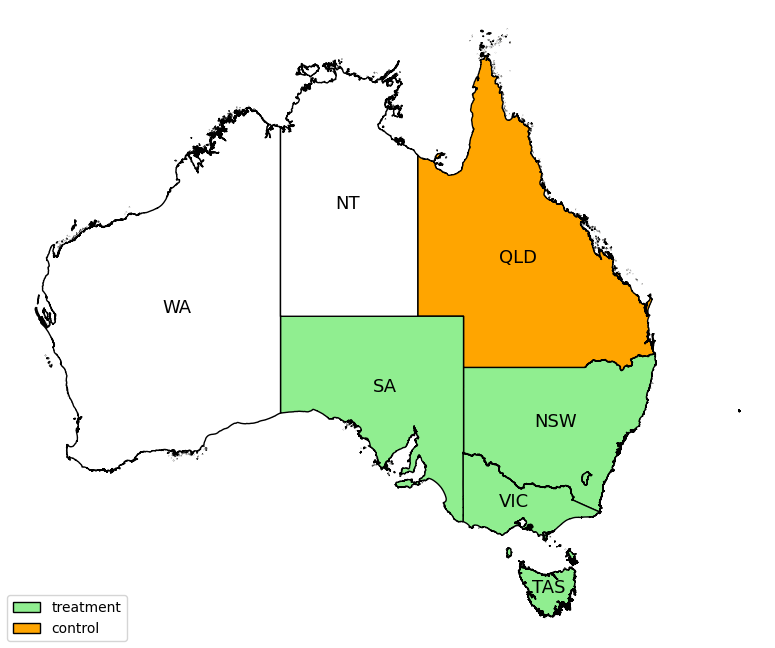
\includegraphics[width=0.4\textwidth]{map.png}
    \caption{Map of Australia showing treatment and control regions}
    \label{fig:map}
\end{figure}

\begin{figure}[ht]
    \centering
    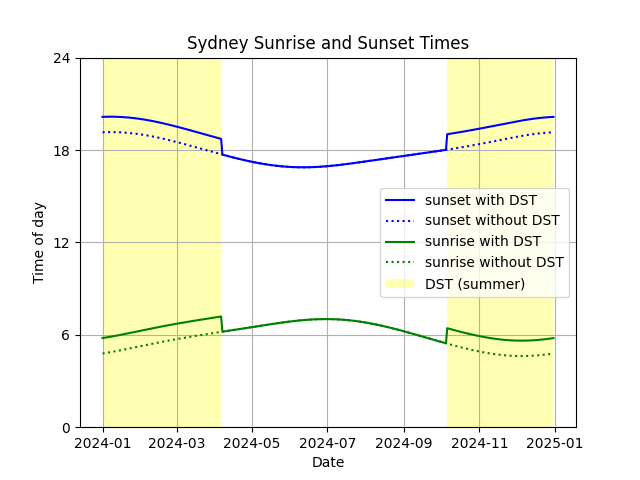
\includegraphics[width=\textwidth]{sunrise.png}
    \caption[Effect of \acs{DST} on apparent sunrise and sunset times in Sydney]{Effect of \acs{DST} on apparent sunrise and sunset times in Sydney. Note that since Australia is in the southern hemisphere, summer and \acs{DST} occur at the start and end of the calendar year.}
    \label{fig:sunrise plot}
\end{figure}

\begin{figure}[ht]
    \centering
    \begin{subfigure}[t]{0.45\textwidth} 
        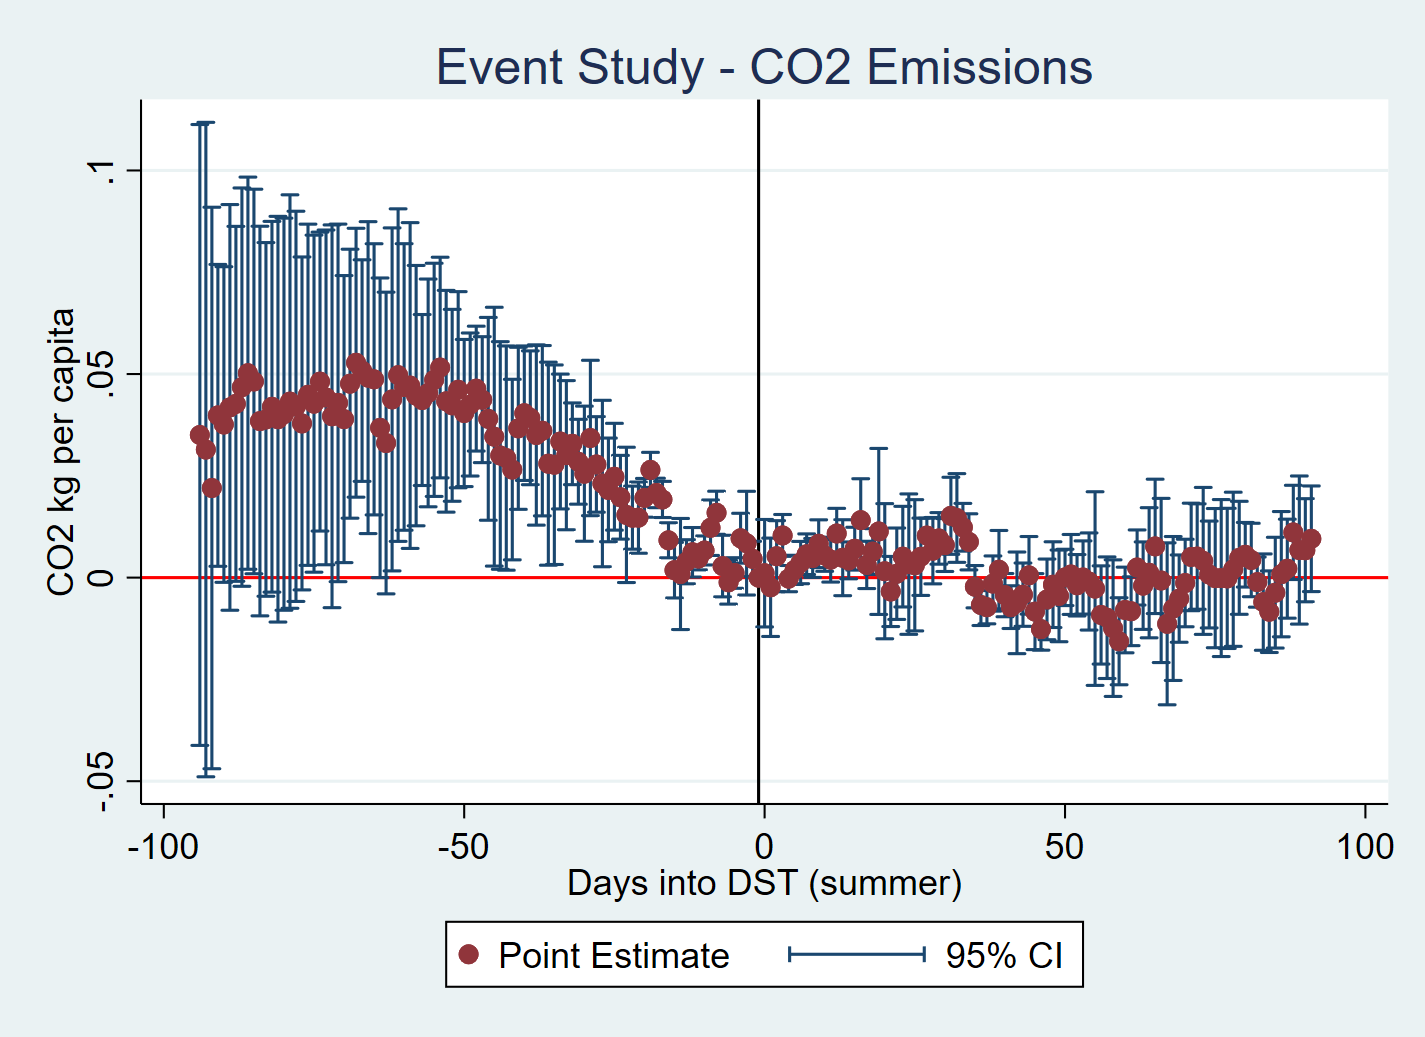
\includegraphics[width=\textwidth]{EventStudy-CO2.png}
        % Subcaption for the first image
        \caption{\acs{DiD} Event study plot for CO2 Emissions}
        \label{fig:dd event study co2}
    \end{subfigure}
    \hfill 
    \begin{subfigure}[t]{0.45\textwidth} 
        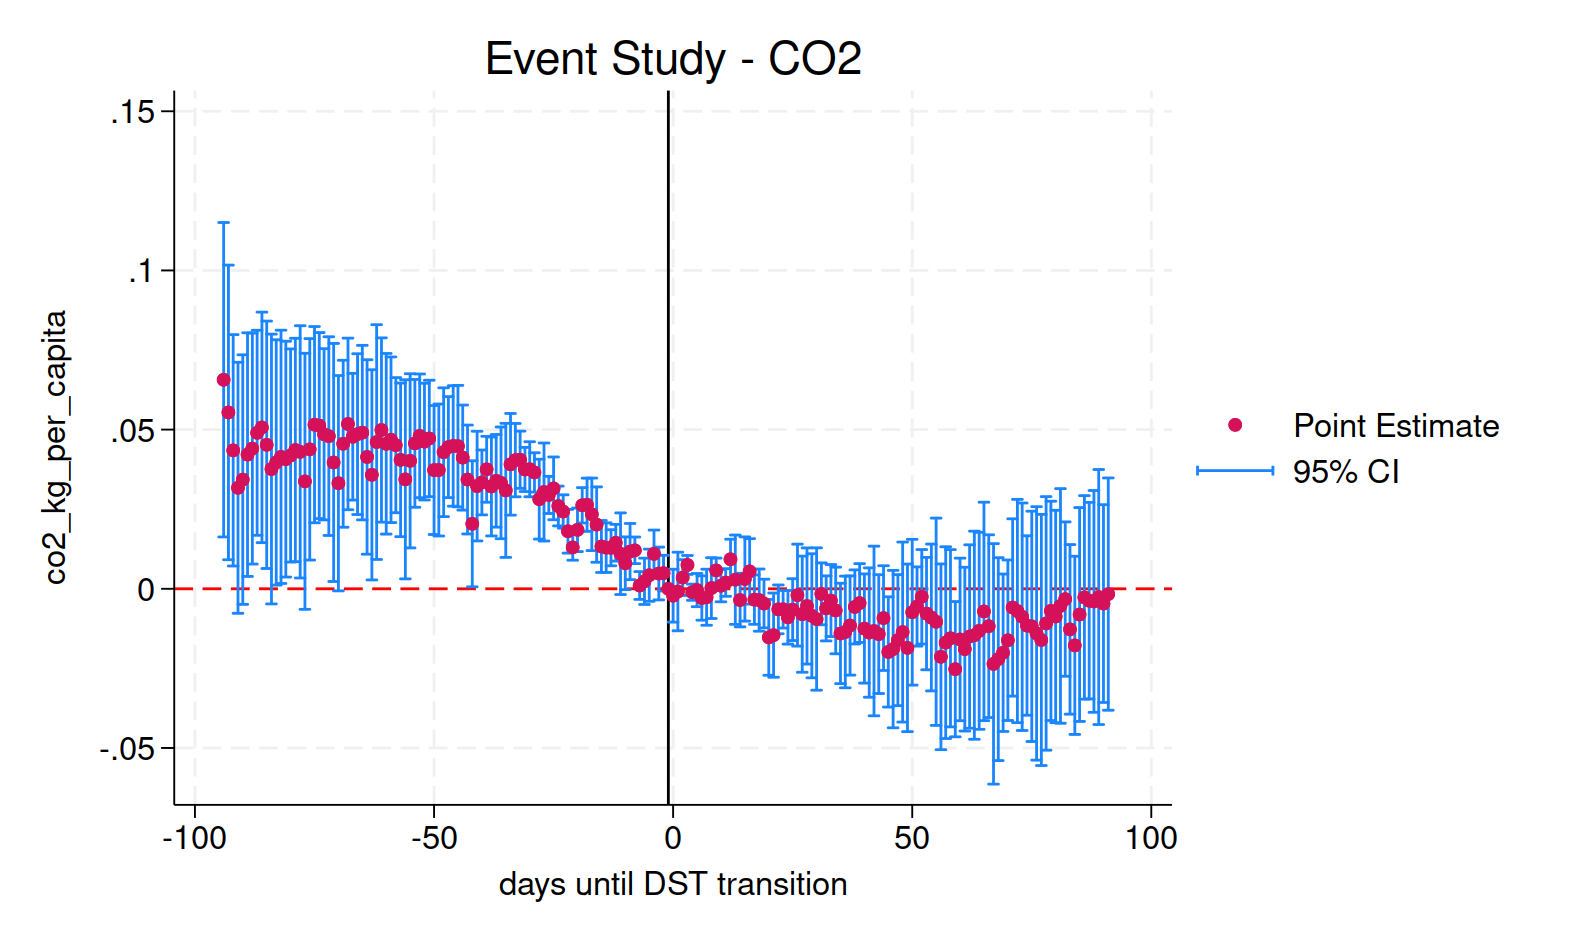
\includegraphics[width=\textwidth]{EventStudy-Elec.png} 
        \caption{\acs{DiD} Event study plot for CO2 Emissions} % Subcaption for the second image
        \label{fig:dd event study elec}
    \end{subfigure}
    % Shared caption for both subfigures
   \caption[Event study plots for \acs{DiD}]{Event study plots for \acs{DiD}. Both forward and backward clock changes are represented on the same plot, with the latter flipped accordingly. Summer is on the right of each plot, winter on the left. A common prior trend does not exist, because the points on the left half of each plot are jointly significant. The right half of each plot is close to zero, suggesting some sort of common post trend. However this is the treatment period, so such a result cannot be used to justify a \ac{DiD} to the control region.}
    \label{fig:dd event study}
\end{figure}


\begin{figure}[ht]
    \centering
    \begin{subfigure}[t]{0.45\textwidth} 
        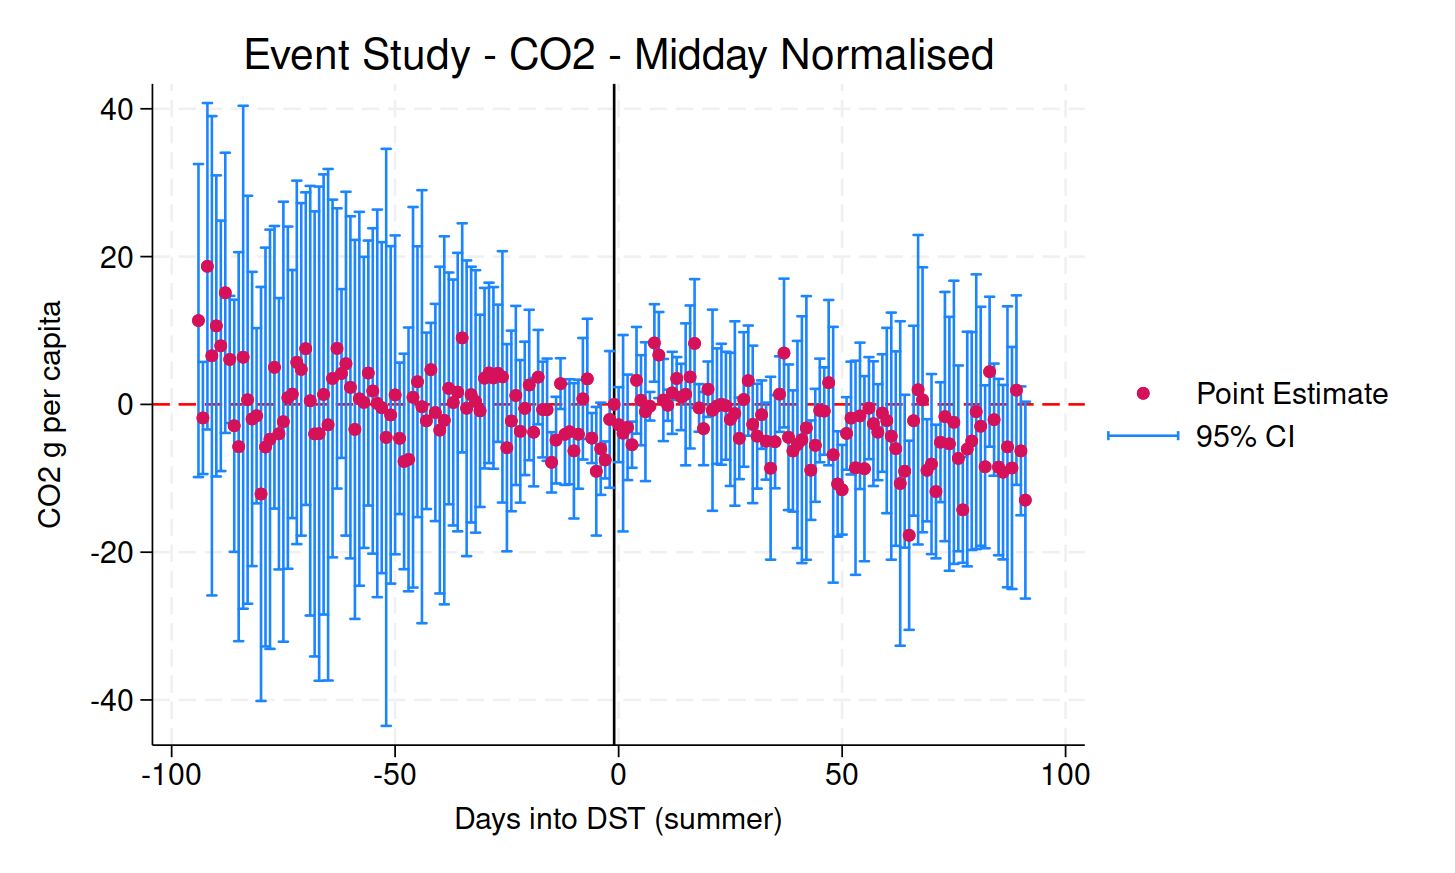
\includegraphics[width=\textwidth]{EventStudy-MiddayCO2.png}
        % Subcaption for the first image
        \caption{\acs{DDD} Event study plot for CO2 Emissions}
        \label{fig:ddd event study co2}
    \end{subfigure}
    \hfill 
    \begin{subfigure}[t]{0.45\textwidth} 
        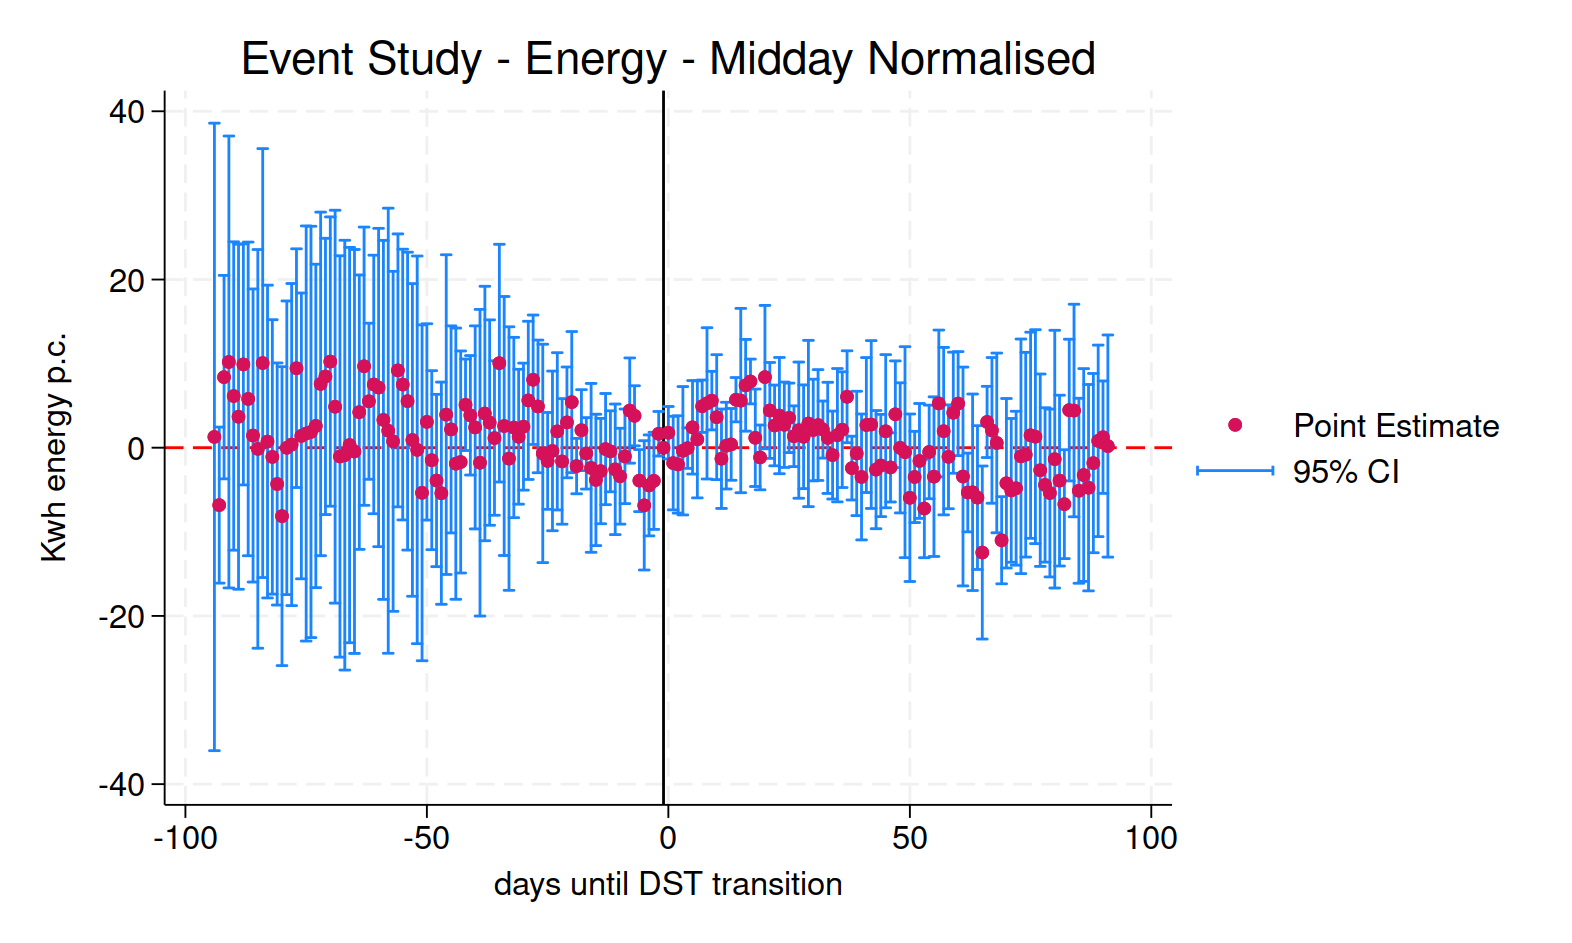
\includegraphics[width=\textwidth]{EventStudy-MiddayElec.png} 
        \caption{\acs{DDD} Event study plot for CO2 Emissions} % Subcaption for the second image
        \label{fig:ddd event study elec}
    \end{subfigure}
    % Shared caption for both subfigures
    \caption[Event study plots for \acs{DiD}]{Event study plots for \acs{DiD}. For each day, for each region, the average value of emission or energy during 12:00-14:30 was calculated, and subtracted from the value for all intervals. Then the same procedure was applied as for Figure \ref{fig:dd event study}. The left half of each plot is approximately zero, so there is a common prior trend. The right half is approximately zero, so there is a null result.} 
    \label{fig:ddd event study}
\end{figure}


\begin{figure}[ht]
    \centering
    \begin{subfigure}[t]{0.45\textwidth} 
        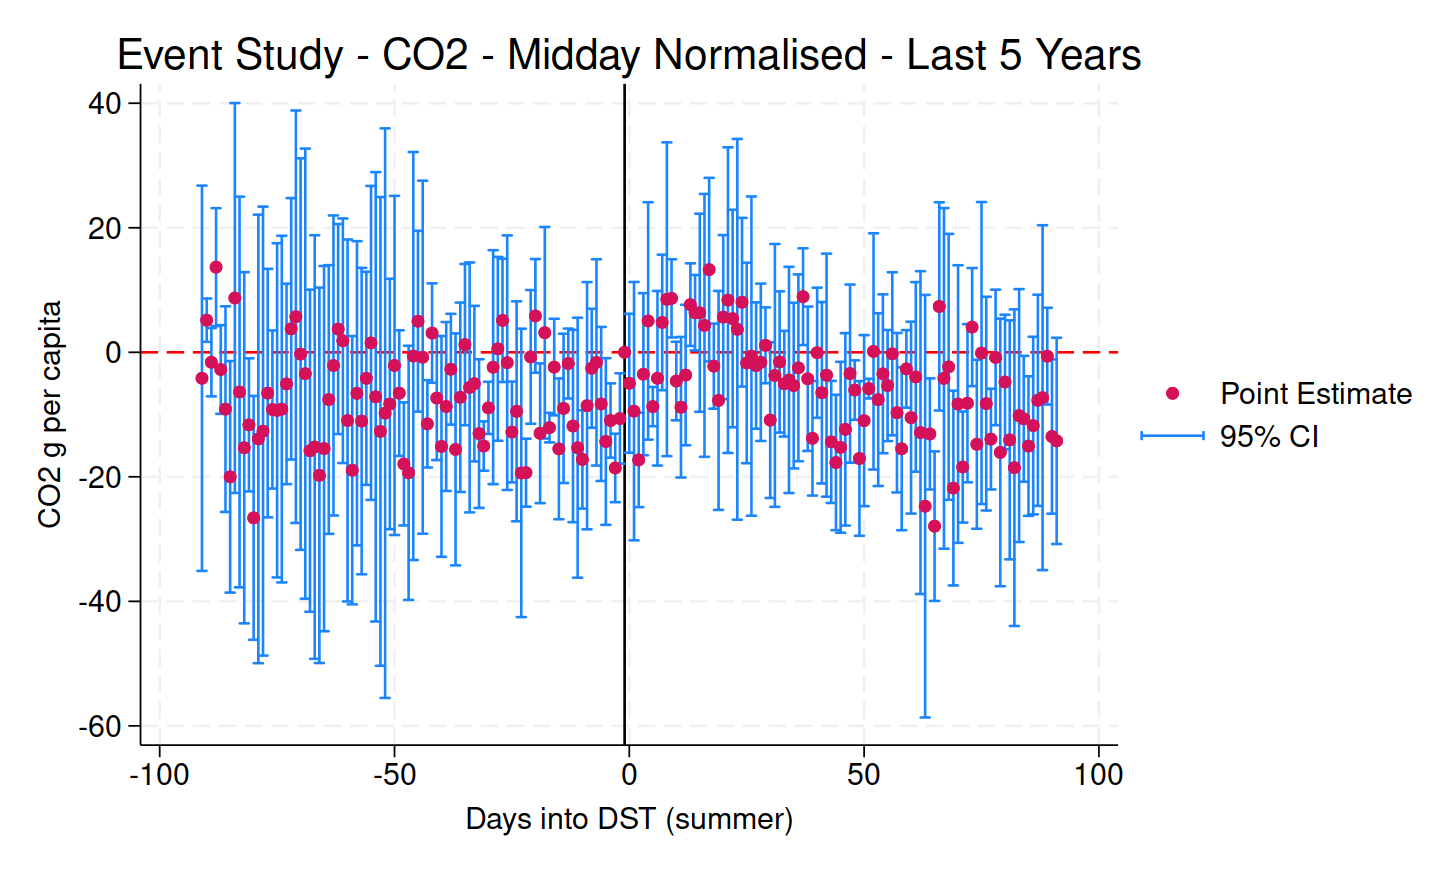
\includegraphics[width=\textwidth]{EventStudy-MiddayCO2-5year.png}
        % Subcaption for the first image
        \caption{\acs{DDD} Event study plot for CO2 Emissions - Last 5 years}
        \label{fig:ddd event study co2 - Last 5}
    \end{subfigure}
    \hfill 
    \begin{subfigure}[t]{0.45\textwidth} 
        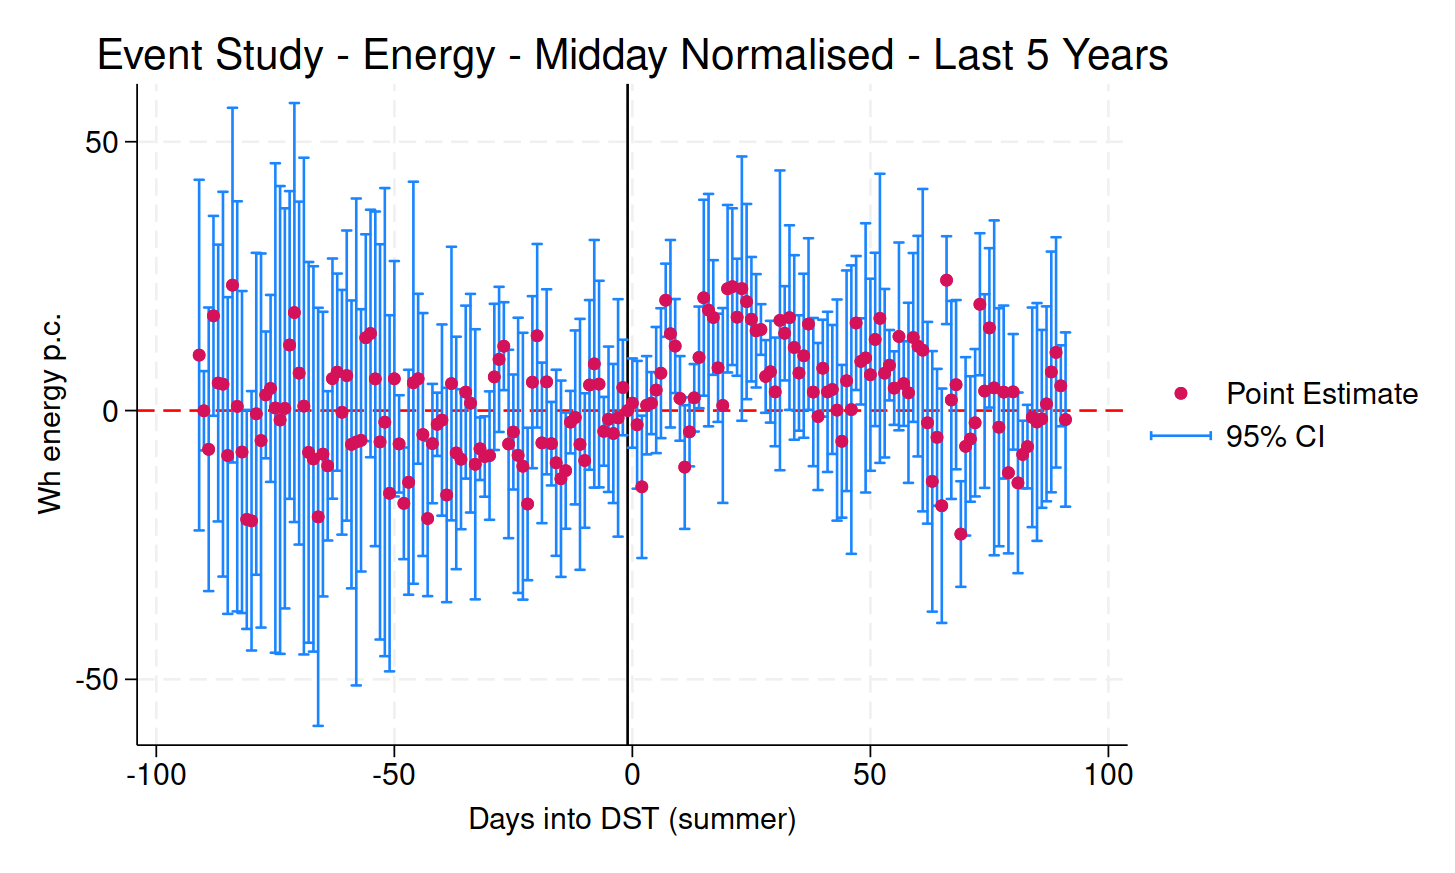
\includegraphics[width=\textwidth]{EventStudy-MiddayElec-5year.png} 
        \caption{\acs{DDD} Event study plot for Electricity consumption - Last 5 years} % Subcaption for the second image
        \label{fig:ddd event study elec - Last 5}
    \end{subfigure}
    % Shared caption for both subfigures
    \caption[Event study plots for \acs{DDD} using last 5 years]{Event study plots for \acs{DDD}. Using only the last 5 years of our data we see the size of our coefficients increase relative to the errors. However, our DDD regression results still remain insignificant at the 5\% level. \ref{DDD-Last-5-Results}} 
    \label{fig:ddd event study - Last 5}
\end{figure}

\begin{figure}[ht]
    \centering
    \begin{subfigure}[t]{0.45\textwidth} 
        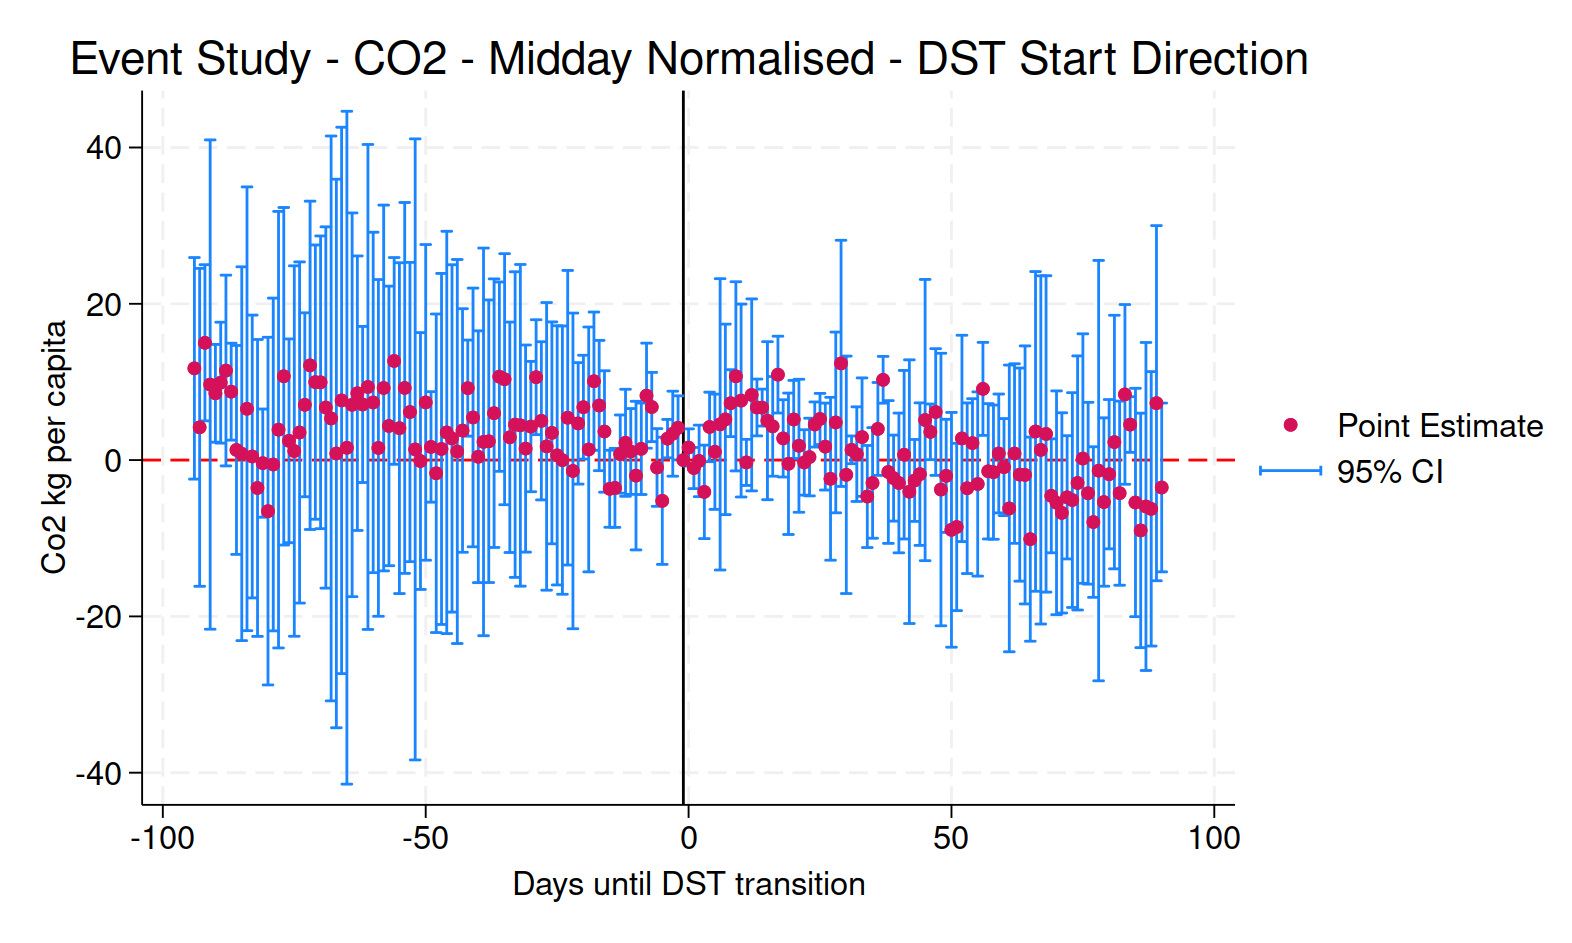
\includegraphics[width=\textwidth]{EventStudy-MiddayCO2-DST-Start.png}
        % Subcaption for the first image
        \caption{\acs{DDD} Event study plot for CO2 Emissions only for the DST start (clock forward)}
        \label{fig:ddd event study co2 start}
    \end{subfigure}
    \hfill 
    \begin{subfigure}[t]{0.45\textwidth} 
        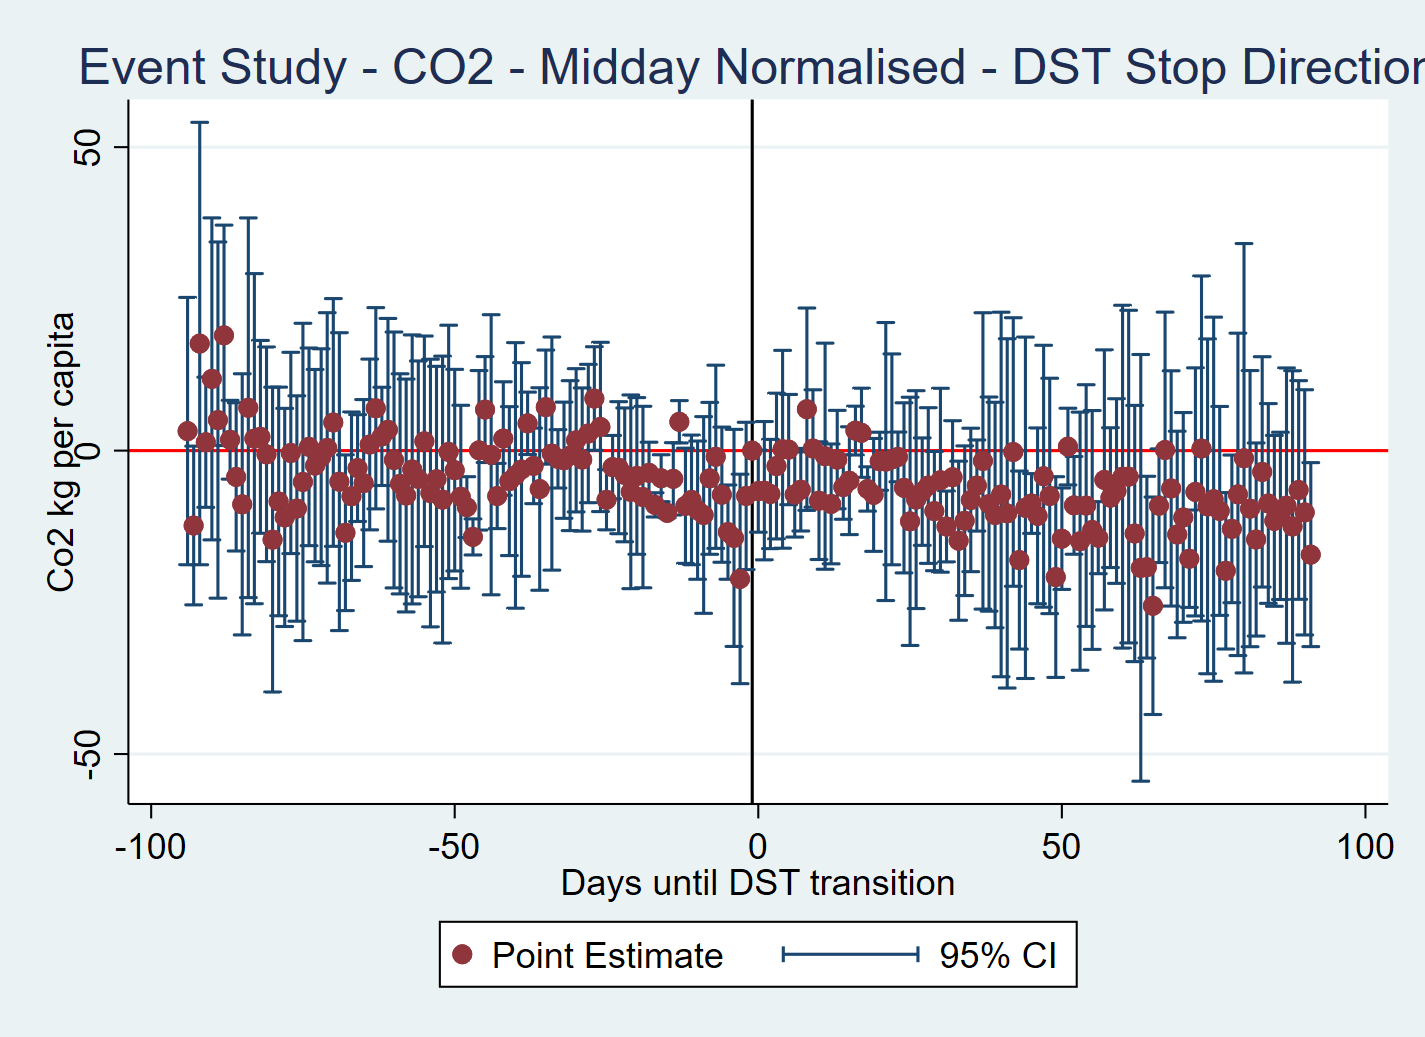
\includegraphics[width=\textwidth]{EventStudy-MiddayCO2-DST-Stop.png}
        \caption{\acs{DDD} Event study plot for CO2 Emissions only for the DST stop (clock backward). The plot chronologically reversed. The data starts in the middle of summer, during \acs{DST} on the right of the plot, and time progresses forwards towards the left. The clocks are moved back on the morning of day -1. Then once the treatment is unapplied, the "Days into \acs{DST}" continues to become more negative, with mid-winter on the far left.} % Subcaption for the second image
        \label{fig:ddd event study co2 stop}
    \end{subfigure}
    % Shared caption for both subfigures
    \caption[Event study plots for \acs{DiD} split by clock change direction]{Event study plots for \acs{DiD}, split by clock direction. This is the same as Figure \ref{fig:ddd event study co2}, but split into clock forward and clock back transitions, as a robustness check. The common prior trend and null result still hold.} 
    \label{fig:ddd event study co2 start stop}
\end{figure}

\begin{figure}[ht]
    \centering
    \begin{subfigure}[t]{0.45\textwidth} 
        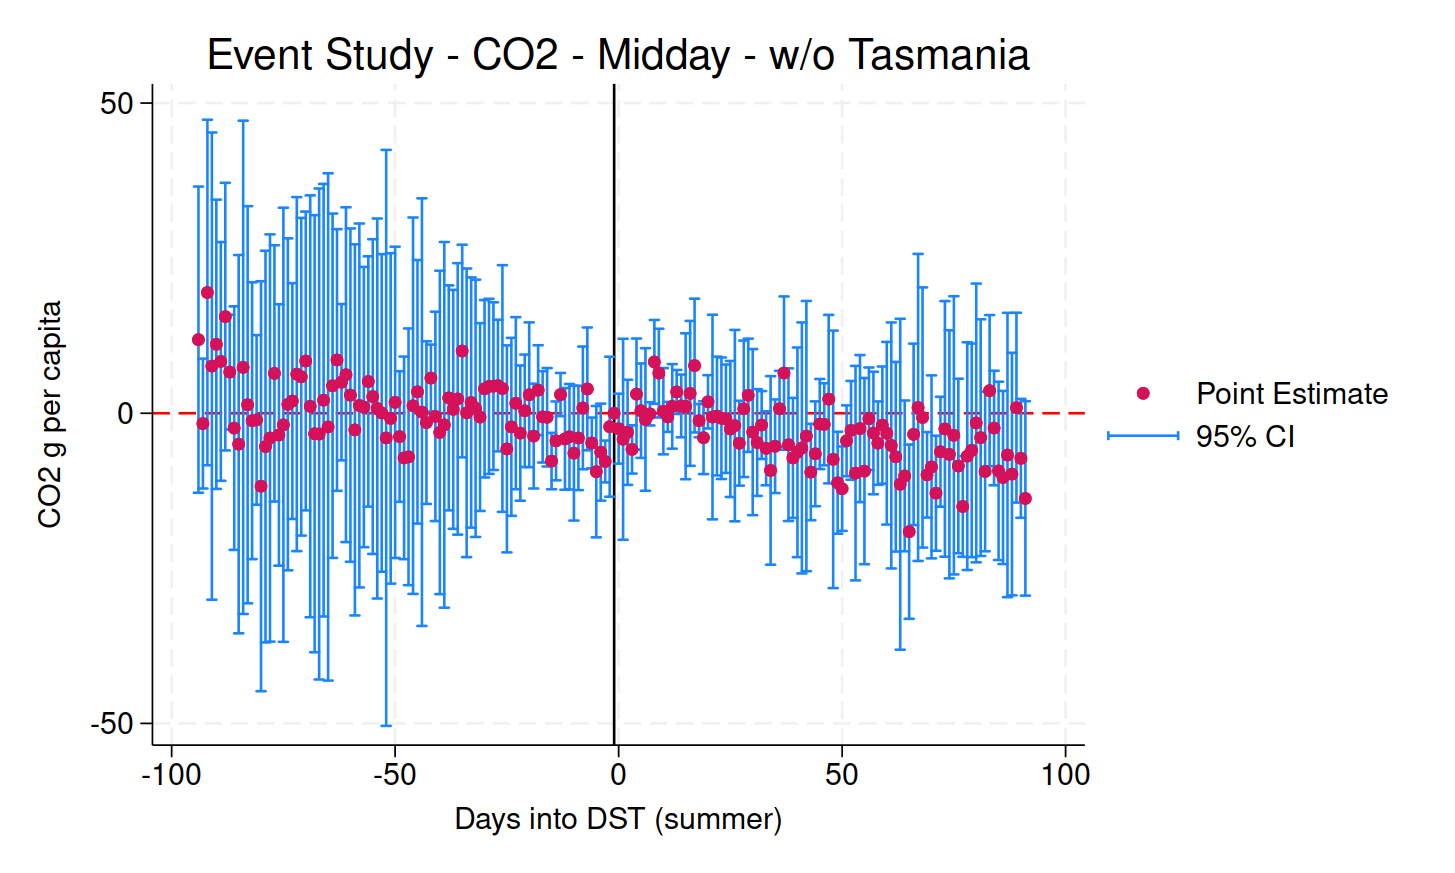
\includegraphics[width=\textwidth]{EventStudy-MiddayCO2-Dropping-Tasmania.png}
        % Subcaption for the first image
        \caption{\acs{DDD} Event study plot for CO2 Emissions when normalising for midday values and dropping Tasmania}
        \label{fig:ddd event study co2 w/o Tas}
    \end{subfigure}
    \hfill 
    \begin{subfigure}[t]{0.45\textwidth} 
        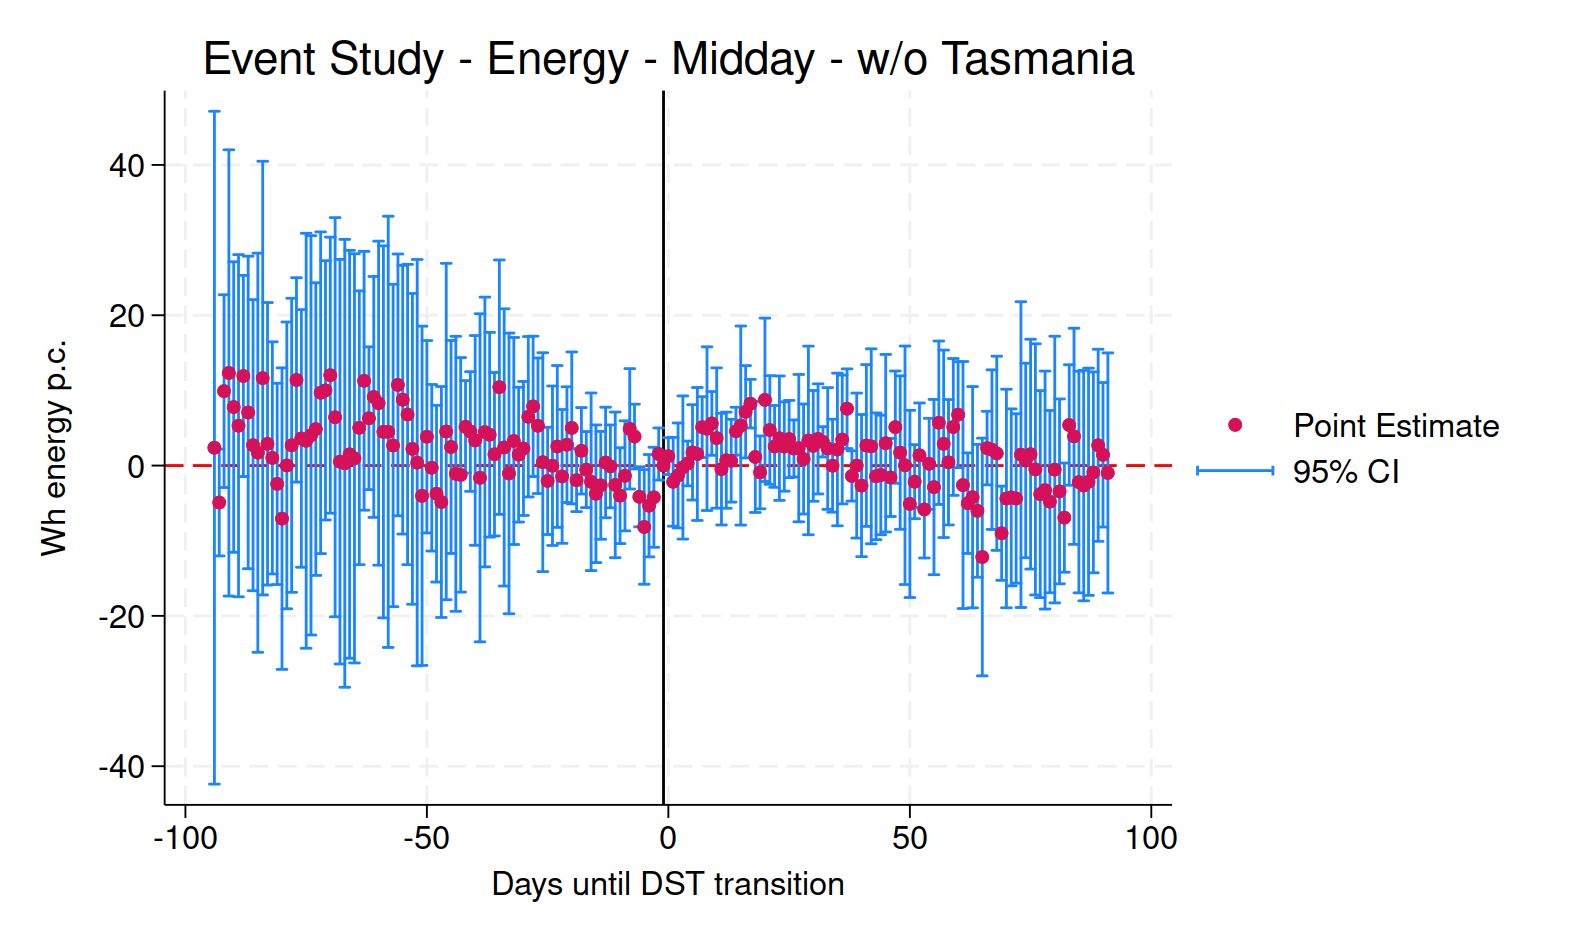
\includegraphics[width=\textwidth]{EventStudy-MiddayElec-Dropping-Tasmania.png}
        \caption{\acs{DDD} Event study plot for Electricity consumption when normalising for midday values and dropping Tasmania} % Subcaption for the second image
        \label{fig:ddd event study Elec w/o Tas}
    \end{subfigure}
    % Shared caption for both subfigures
    \caption[Event study plots for \acs{DDD} without Tasmania]{Event study plots for \acs{DDD}, dropping Tasmania as a robustness check. The common prior trend and null result still hold.} 
    \label{fig:ddd event study w/o Tas}
\end{figure}


\begin{figure}[ht]
    \centering
    \begin{subfigure}[t]{0.45\textwidth} 
        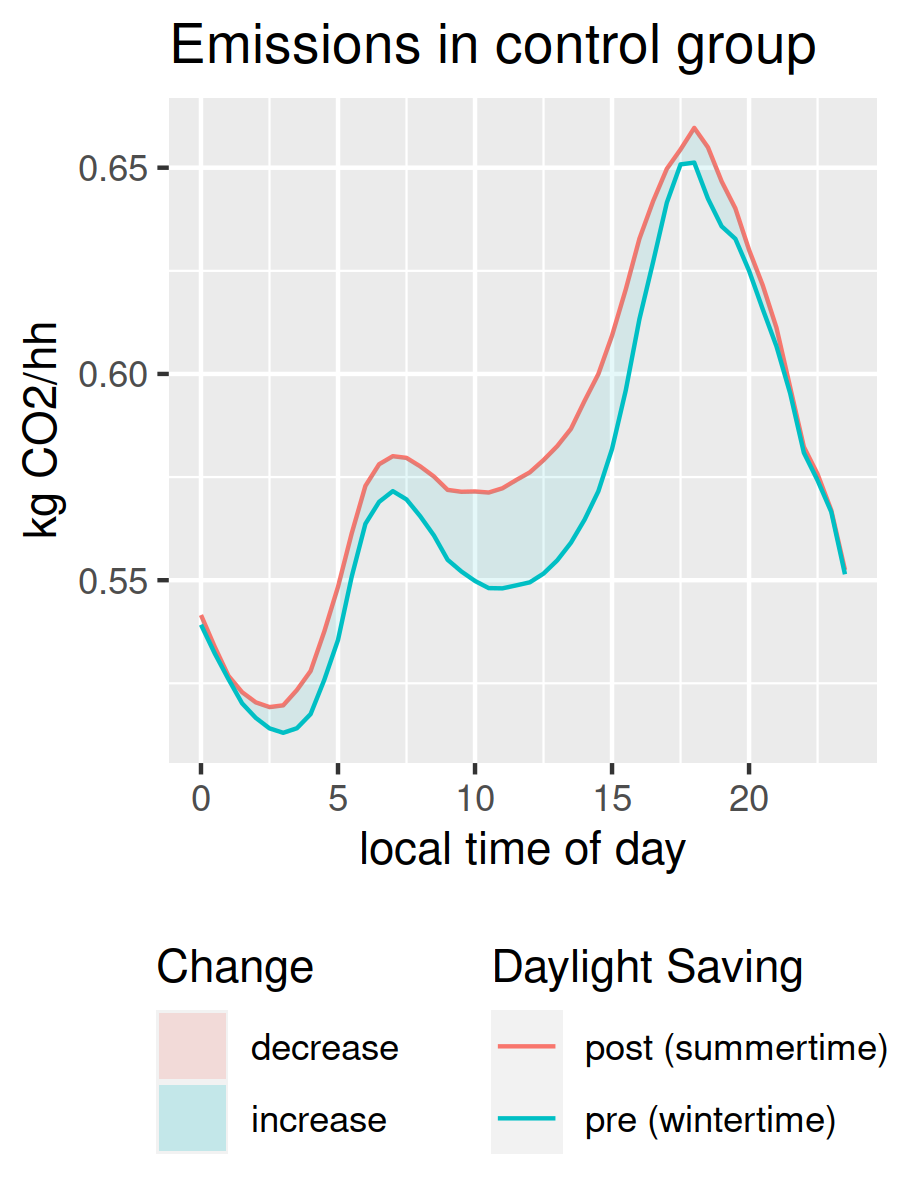
\includegraphics[width=\textwidth]{Images/intraday/co2_kg_per_capita/by-treated/control/hr_local-filled.png}
        % Subcaption for the first image
        \caption{Average intraday emissions in the control region}
        \label{fig:intraday co2 control}
    \end{subfigure}
    \hfill 
    \begin{subfigure}[t]{0.45\textwidth} 
        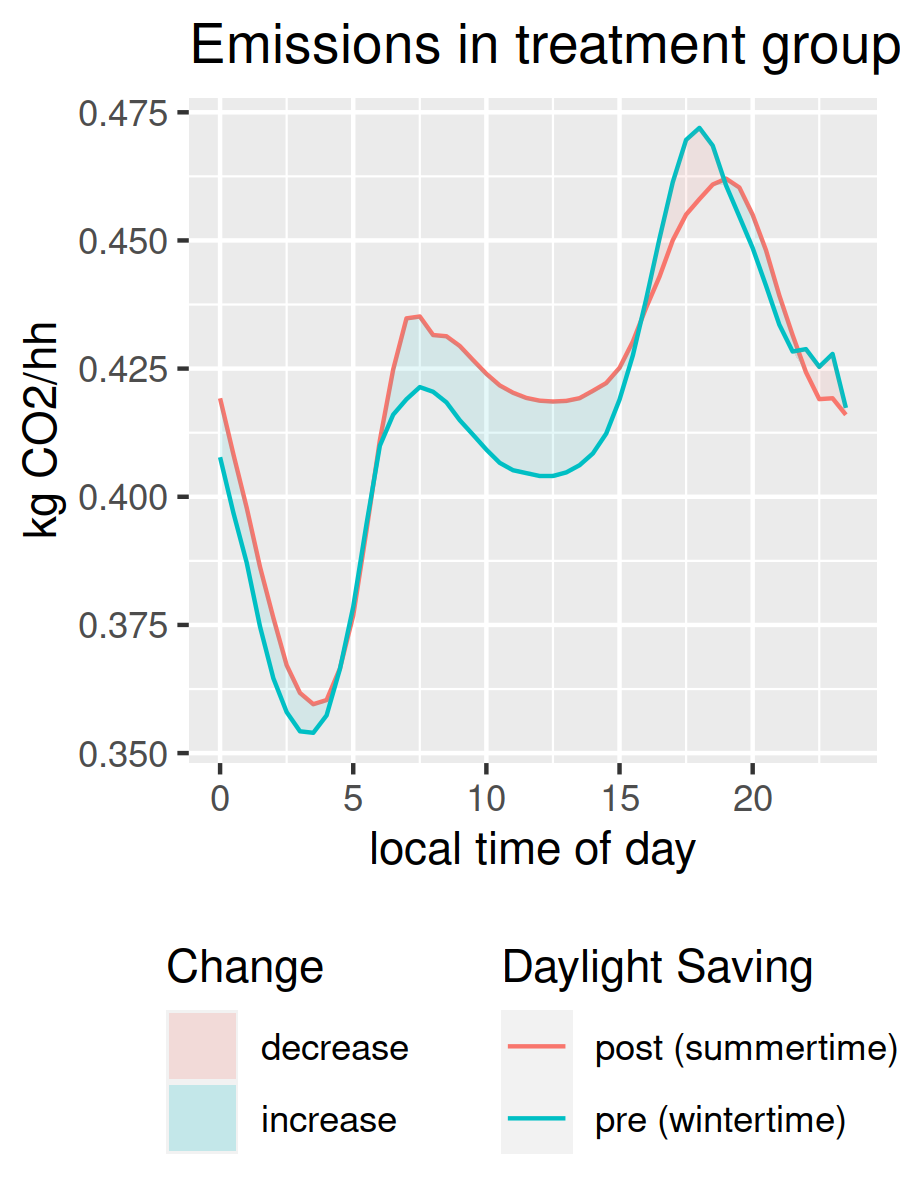
\includegraphics[width=\textwidth]{Images/intraday/co2_kg_per_capita/by-treated/treatment/hr_local-filled.png}
        \caption{Average intraday emissions in the treated regions} % Subcaption for the second image
        \label{fig:intraday co2 treated}
    \end{subfigure}
    % Shared caption for both subfigures
    \caption[Average intraday emissions, with and without \acs{DST}, for treated and control]{Average intraday emissions, with and without \acs{DST}, for treated and control. The fact that there is more of the red (decrease) area and less of the green (increase) for the treated region than the control suggests that \acs{DST} does reduce emissions. However this effect disappears once accounting for controls.} 
    \label{fig:intraday co2}
\end{figure}


\begin{figure}[ht]
    \centering
    \begin{subfigure}[t]{0.45\textwidth} 
        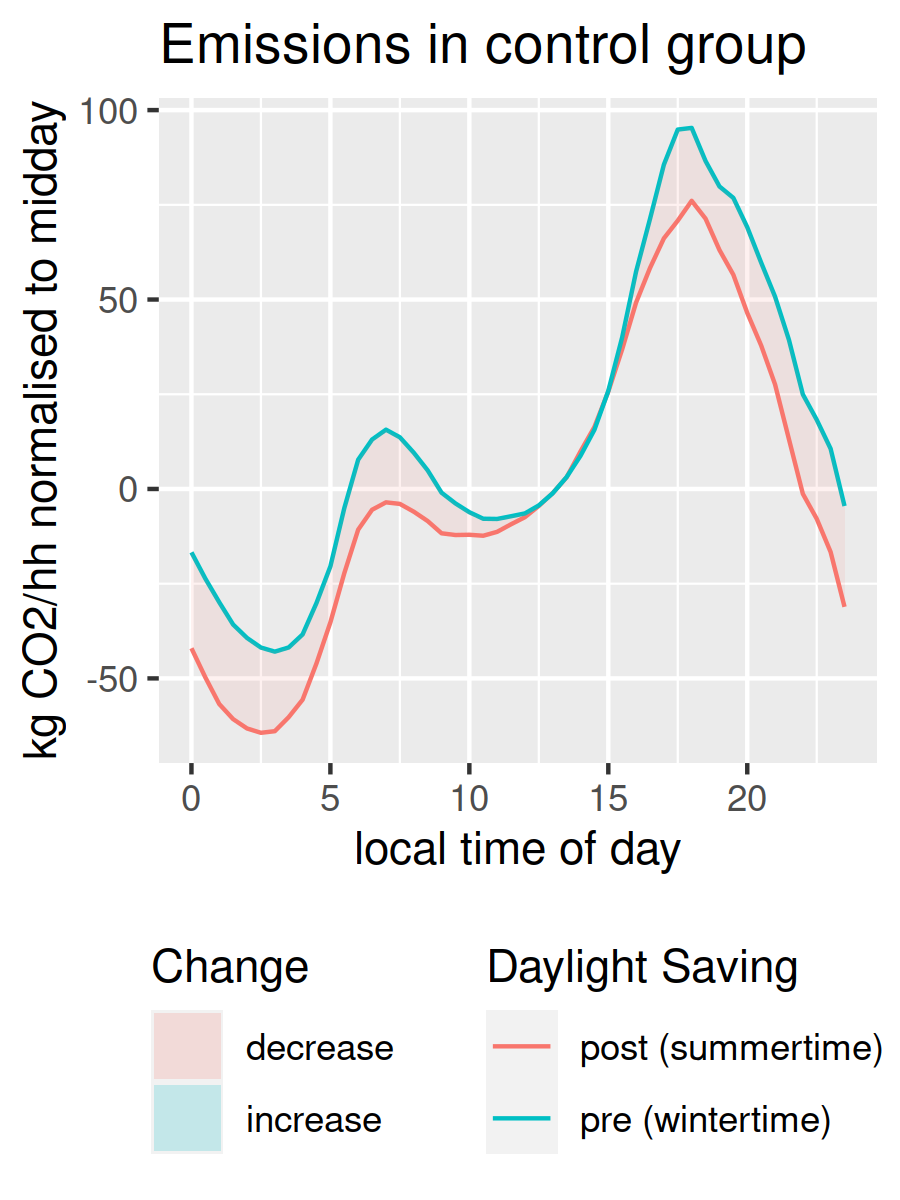
\includegraphics[width=\textwidth]{Images/intraday/co2_g_per_capita_vs_midday/by-treated/control/hr_local-filled.png}
        % Subcaption for the first image
        \caption{Average intraday emissions in the control region}
        \label{fig:intraday co2 control midday}
    \end{subfigure}
    \hfill 
    \begin{subfigure}[t]{0.45\textwidth} 
        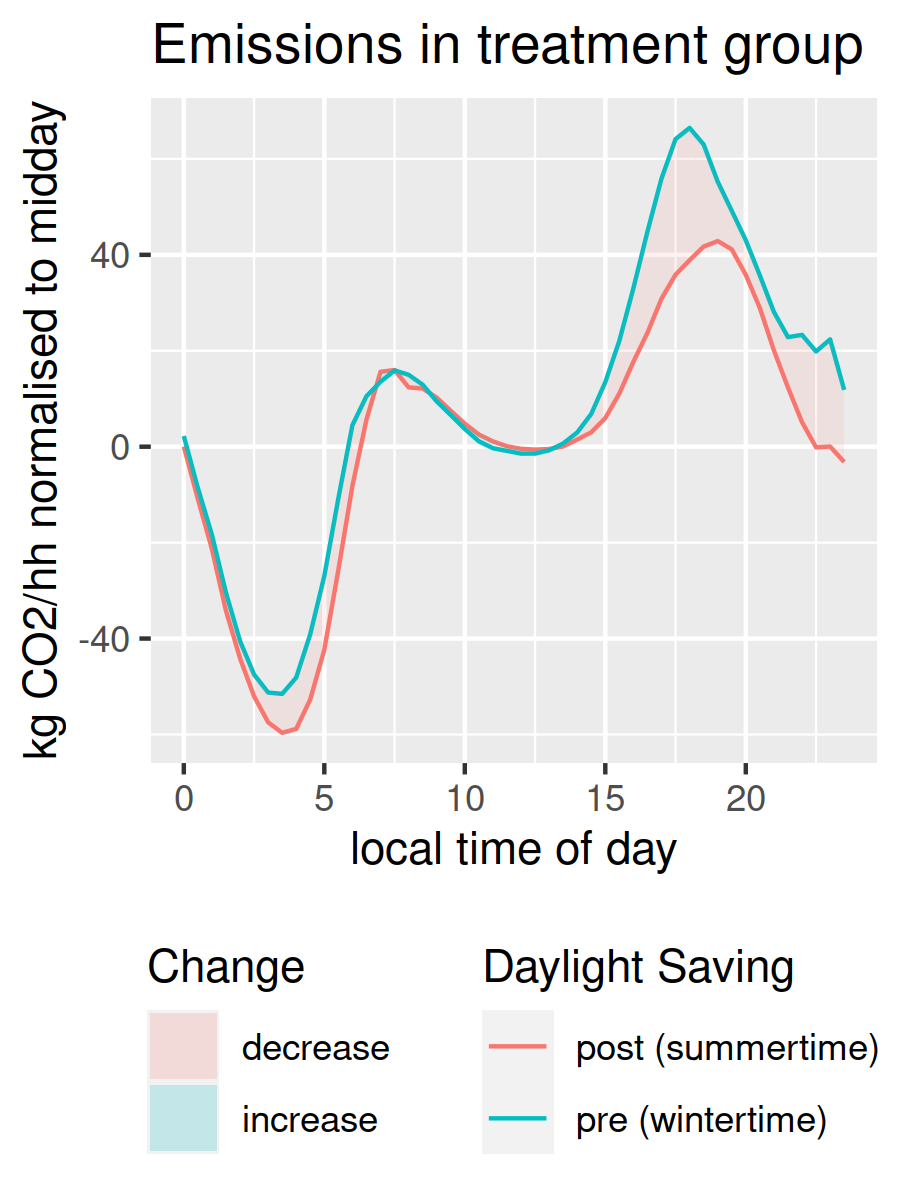
\includegraphics[width=\textwidth]{Images/intraday/co2_g_per_capita_vs_midday/by-treated/treatment/hr_local-filled.png}
        \caption{Average intraday emissions in the treated regions} % Subcaption for the second image
        \label{fig:intraday co2 treated midday}
    \end{subfigure}
    % Shared caption for both subfigures
    \caption[Average intraday emissions, normalising for midday]{Average intraday emissions, normalising for midday. This is the same as Figure \ref{fig:intraday co2}, except the average of the emissions for that day for that region was calculated for 12:00-14:30, and that was subtracted from all intervals for that day. This graphically represents the third differencing step. The fact that the red area (decrease) is larger for the control group suggests that \acs{DST} increases emissions. However once controls are accounted for in the regression, this difference changes sign and becomes statistically insignificant.} 
    \label{fig:intraday co2 midday}
\end{figure}



\begin{landscape}
 \begin{table}[!htbp] \centering
 \caption[Summary Statistics]{\label{tab:summary stats}Summary statistics for all variables, for treatment and control states}
 \begin{tabular}{@{\extracolsep{5pt}}clrccc}
 \hline \hline
    &&&&&\\ [-1.8ex]
  & \multicolumn{1}{l}{Variable} & \multicolumn{1}{r}{[unit]} & \multicolumn{1}{c}{Mean} & \multicolumn{1}{c}{Minimum Value} & \multicolumn{1}{c}{Maximum Value}\\
 \hline
  \parbox[t]{2mm}{\multirow{12}{*}{\rotatebox[origin=l]{90}{\textbf{Treatment}}}}&&&&&\\ [-1.8ex]
   &Population& \([inhabitans]\)& 4,127,718& 505,468 & 8,806,160\\
 &&&&&\\
  &Greenhouse gas emissions per capita& \([kg/half hour]\))& 0.315 & 0.000 & 0.935\\[-1.8ex]
  &&&&&\\
 &Energy production per capita & \([kWh/half hour]\) & 0.533 & 0.001 &41.719\\[-1.8ex]
  &&&&&\\
&Temperature & \([^{\circ}C]\) & 20.97 & 7.20 &46.40\\[-1.8ex]
  &&&&&\\
 &Solar exposure& \([kWh/m^2]\) & 4.75 & 0.11& 9.80\\[-1.8ex]
  &&&&&\\
 &Wind& \([km/h]\) & 16.09 & 0.00 & 51.50\\[-1.8ex]
  &&&&&\\
 &Holiday& \([\% of days]\) &3.41 &3.15 &3.57\\[-1.8ex]
  &&&&&\\
 &Weekend& \([\% of days]\) &0.29&&\\
 \hline
  \parbox[t]{2mm}{\multirow{12}{*}{\rotatebox[origin=l]{90}{\textbf{Control}}}}&&&&&\\ [-1.8ex]
   &Population& \([inhabitans]\)&4,870,395 &4,350,135 &5,459,413\\
  &&&&&\\
 &Greenhouse gas emissions per capita& \([kg/half hour]\)& 0.591 & 0.277 & 0.911\\[-1.8ex]
  &&&&&\\
    &Energy production per capita & \([kWh/half hour]\) & 0.656 & 0.375 & 1.027\\[-1.8ex]
  &&&&&\\
 &Temperature & \([^{\circ}C]\) & 26.64 & 12.60& 41.20\\[-1.8ex]
  &&&&&\\
 &Solar exposure& \([kWh/m^2]\) & 6.13 & 0.50 & 9.27 \\[-1.8ex]
  &&&&&\\
 &Wind& \([km/h]\) & 16.37 & 3.60 &41.00\\[-1.8ex]
  &&&&&\\
 &Holiday& \([\% of days]\) &3.27& 3.27& 3.27\\[-1.8ex]
  &&&&&\\
 &Weekend& \([\% of days]\) &0.29&&\\[-1.8ex]
  &&&&&\\
 \hline
 \end{tabular}
 \end{table}
 \end{landscape}

\def\sym#1{\ifmmode^{#1}\else\(^{#1}\)\fi}

\begin{table}[!htbp] \centering 
  \caption{CO2 and Electricity Consumption Results - DiD} 
  \label{Main-DiD-Results} 
\small 
\def\sym#1{\ifmmode^{#1}\else\(^{#1}\)\fi}
\begin{tabular}{l*{4}{c}}
\\[-1.8ex]\hline 
\hline \\[-1.8ex] 
 & \multicolumn{4}{c}{\textit{Dependent variable:}} \\ 
\cline{2-5} 
\\[-1.8ex] &\multicolumn{1}{c}{kg CO2 p.c.}&\multicolumn{1}{c}{kWh energy p.c.}&\multicolumn{1}{c}{Kg CO2 p.c.}&\multicolumn{1}{c}{kWh energy p.c.}\\ 
\\[-1.8ex] & \multicolumn{1}{c}{(1)} & \multicolumn{1}{c}{(2)} & \multicolumn{1}{c}{(3)} & \multicolumn{1}{c}{(4)}\\ 
\hline \\[-1.8ex] 
Treatment &      -0.133\sym{*}  &      -0.180\sym{**} &      -0.144\sym{**} &      -0.215\sym{***}\\
                    &    (0.0391)         &    (0.0284)         &    (0.0281)         &    (0.0198)         \\
[1em]
Post &      0.0243\sym{***}&      0.0317\sym{***}&      0.0263         &      0.0315         \\
                    &  (1.50e-14)         &  (6.03e-15)         &    (0.0174)         &    (0.0174)         \\
[1em]
Treatment $\times$ Post &     -0.0330\sym{**} &     -0.0568\sym{**} &     -0.0181         &     -0.0235         \\
                    &   (0.00663)         &   (0.00920)         &    (0.0222)         &    (0.0161)         \\
[1em]
Weekend &                     &                     &     -0.0338\sym{***}&     -0.0462\sym{***}\\
                    &                     &                     &   (0.00132)         &   (0.00181)         \\
[1em]
Public Holiday &                     &                     &     -0.0378\sym{**} &     -0.0498\sym{***}\\
                    &                     &                     &   (0.00556)         &   (0.00387)         \\
[1em]
Temperature &                     &                     &     -0.0109         &     -0.0250         \\
                    &                     &                     &    (0.0142)         &    (0.0168)         \\
[1em]
Temperature$^2$ &                     &                     &    0.000272         &    0.000521         \\
                    &                     &                     &  (0.000235)         &  (0.000289)         \\
[1em]
Solar Exposure &                     &                     &    -0.00422         &    -0.00815         \\
                    &                     &                     &   (0.00631)         &   (0.00600)         \\
[1em]
Wind$^3$ &                     &                     &     -0.0594         &     0.00417         \\
                    &                     &                     &    (0.0249)         &    (0.0119)         \\
[1em]
Constant            &       0.576\sym{***}&       0.656\sym{***}&       0.736\sym{*}  &       1.008\sym{*}  \\
                    &  (1.41e-14)         &  (6.97e-15)         &     (0.215)         &     (0.265)         \\
\hline
r2                  &       0.152         &       0.326         &       0.213         &       0.378         \\
r2\_a                &       0.152         &       0.326         &       0.213         &       0.378         \\
\hline\hline
\multicolumn{5}{l}{Note: Errors clustered by region, weighted by population.} \\
\multicolumn{2}{l}{Dependent variables are measured per half hour.} \\
\multicolumn{5}{l}{\footnotesize Standard errors in parentheses}\\
\multicolumn{5}{l}{\footnotesize \sym{*} \(p<0.05\), \sym{**} \(p<0.01\), \sym{***} \(p<0.001\)}\\
\end{tabular}
\end{table}

\def\sym#1{\ifmmode^{#1}\else\(^{#1}\)\fi}

\begin{table}[!htbp] \centering 
  \caption{Results For CO2 and Electricity Consumption DDD With Controls} 
  \label{Main-DDD-Results} 
\small 
\begin{tabular}{@{\extracolsep{5pt}}lD{.}{.}{-3} D{.}{.}{-3} } 
\\[-1.8ex]\hline 
\hline \\[-1.8ex] 
 & \multicolumn{2}{c}{\textit{Dependent variable:}} \\ 
\cline{2-3} 
\\[-1.8ex] & \multicolumn{1}{c}{Kg CO2 p.c.} & \multicolumn{1}{c}{Kwh energy consumption p.c.} \\ 
\\[-1.8ex] & \multicolumn{1}{c}{(1)} & \multicolumn{1}{c}{(2)}\\ 
\hline \\[-1.8ex]
Treatment&      -0.134\sym{*}  &      -0.216\sym{***}\\
                    &    (0.0306)         &    (0.0216)         \\
[1em]
Post&      0.0605\sym{*}  &      0.0788\sym{*}  \\
                    &    (0.0174)         &    (0.0174)         \\
[1em]
Treatment $\times$ Post &     -0.0303         &     -0.0401         \\
                    &    (0.0186)         &    (0.0196)         \\
[1em]
Not Midday &      0.0272\sym{***}&      0.0143\sym{***}\\
                    &  (8.78e-13)         &  (1.00e-12)         \\
[1em]
Treatment $\times$ Not Midday &     -0.0115         &    0.000875         \\
                    &   (0.00874)         &   (0.00608)         \\
[1em]
Post $\times$ Not Midday &     -0.0382\sym{***}&     -0.0529\sym{***}\\
                    &  (2.00e-12)         &  (2.33e-12)         \\
[1em]
Treatment $\times$ Post $\times$ Not Midday &      0.0136         &      0.0185         \\
                    &    (0.0129)         &    (0.0110)         \\
[1em]
Weekend    &     -0.0338\sym{***}&     -0.0462\sym{***}\\
                    &   (0.00132)         &   (0.00181)         \\
[1em]
Public Holiday &     -0.0378\sym{**} &     -0.0498\sym{***}\\
                    &   (0.00556)         &   (0.00387)         \\
[1em]
Temperature&     -0.0109         &     -0.0250         \\
                    &    (0.0142)         &    (0.0168)         \\
[1em]
Temperature2 &    0.000272         &    0.000521         \\
                    &  (0.000235)         &  (0.000289)         \\
[1em]
Solar Exposure&    -0.00422         &    -0.00815         \\
                    &   (0.00631)         &   (0.00600)         \\
[1em]
Wind3 &     -0.0594         &     0.00417         \\
                    &    (0.0249)         &    (0.0119)         \\
[1em]
Constant            &       0.712\sym{*}  &       0.995\sym{*}  \\
                    &     (0.215)         &     (0.265)         \\
\hline
r2                  &       0.214         &       0.380         \\
r2\_a                &       0.214         &       0.380         \\
\hline \\[-1.8ex] 
\hline 
\hline \\[-1.8ex] 
\multicolumn{2}{l}{Note: Errors clustered by region, weighted by population} \\ \multicolumn{2}{l}{$^{*}$p$<$0.1; $^{**}$p$<$0.05; $^{***}$p$<$0.01} \\ 
\end{tabular} 
\end{table} 
\def\sym#1{\ifmmode^{#1}\else\(^{#1}\)\fi}

\begin{table}[!htbp] \centering 
  \caption{Results For CO2 and Electricity Consumption Base DDD Without Controls} 
  \label{DDD-WO-Controls-Results} 
\small 
\begin{tabular}{@{\extracolsep{5pt}}lD{.}{.}{-3} D{.}{.}{-3} } 
\\[-1.8ex]\hline 
\hline \\[-1.8ex] 
 & \multicolumn{2}{c}{\textit{Dependent variable:}} \\ 
\cline{2-3} 
\\[-1.8ex] & \multicolumn{1}{c}{Kg CO2 p.c.} & \multicolumn{1}{c}{Kwh energy consumption p.c.} \\ 
\\[-1.8ex] & \multicolumn{1}{c}{(1)} & \multicolumn{1}{c}{(2)}\\ 
\hline \\[-1.8ex]
\hline
Treatment &      -0.123\sym{*}  &      -0.180\sym{**} \\
                    &    (0.0435)         &    (0.0256)         \\
[1em]
Post &      0.0585\sym{***}&      0.0790\sym{***}\\
                    &  (1.26e-13)         &  (2.01e-13)         \\
[1em]
Treatment $\times$ Post &     -0.0451\sym{***}&     -0.0734\sym{**} \\
                    &   (0.00506)         &    (0.0142)         \\
[1em]
Not Midday &      0.0272\sym{***}&      0.0143\sym{***}\\
                    &  (1.28e-13)         &  (1.27e-13)         \\
[1em]
Treatment $\times$ Not Midday &     -0.0115         &    0.000858         \\
                    &   (0.00875)         &   (0.00608)         \\
[1em]
Post $\times$ Not Midday &     -0.0382\sym{***}&     -0.0529\sym{***}\\
                    &  (1.67e-13)         &  (2.29e-13)         \\
[1em]
Treatment $\times$ Post $\times$ Not Midday &      0.0136         &      0.0185         \\
                    &    (0.0129)         &    (0.0110)         \\
[1em]
Constant            &       0.552\sym{***}&       0.643\sym{***}\\
                    &  (1.28e-13)         &  (1.34e-13)         \\
\hline
r2                  &       0.153         &       0.328         \\
r2\_a                &       0.153         &       0.328         \\
\hline\hline
\multicolumn{3}{l}{\footnotesize Standard errors in parentheses}\\
\multicolumn{3}{l}{\footnotesize \sym{*} \(p<0.05\), \sym{**} \(p<0.01\), \sym{***} \(p<0.001\)}\\
\end{tabular}
\end{table}
\def\sym#1{\ifmmode^{#1}\else\(^{#1}\)\fi}

\begin{table}[!htbp] \centering 
  \caption{Results For ln(CO2) and ln(Electricity Consumption) DDD With Controls} 
  \label{DDD-ln-Results} 
\small 
\begin{tabular}{@{\extracolsep{5pt}}lD{.}{.}{-3} D{.}{.}{-3} } 
\\[-1.8ex]\hline 
\hline \\[-1.8ex] 
 & \multicolumn{2}{c}{\textit{Dependent variable:}} \\ 
\cline{2-3} 
\\[-1.8ex] & \multicolumn{1}{c}{ln(Kg CO2 p.c.)} & \multicolumn{1}{c}{ln(Kwh energy consumption p.c.)} \\ 
\\[-1.8ex] & \multicolumn{1}{c}{(1)} & \multicolumn{1}{c}{(2)}\\ 
\hline \\[-1.8ex]
Treatment &      -0.351\sym{*}  &      -0.409\sym{***}\\
                    &     (0.124)         &    (0.0464)         \\
[1em]
Post &       0.130         &       0.108\sym{*}  \\
                    &    (0.0509)         &    (0.0280)         \\
[1em]
Treatment $\times$ Post &     -0.0490         &     -0.0566         \\
                    &    (0.0524)         &    (0.0337)         \\
[1em]
Not Midday &      0.0569\sym{***}&      0.0224\sym{***}\\
                    &  (3.57e-12)         &  (1.43e-12)         \\
[1em]
Treatment $\times$ Not Midday &     0.00157         &      0.0116         \\
                    &    (0.0291)         &    (0.0131)         \\
[1em]
Post $\times$ Not Midday &     -0.0671\sym{***}&     -0.0764\sym{***}\\
                    &  (6.78e-12)         &  (3.25e-12)         \\
[1em]
Treatment $\times$ Post $\times$ Not Midday&      0.0186         &      0.0153         \\
                    &    (0.0311)         &    (0.0242)         \\
[1em]
Weekend &     -0.0774\sym{**} &     -0.0947\sym{***}\\
                    &    (0.0124)         &    (0.0109)         \\
[1em]
Public Holiday &     -0.0900\sym{*}  &      -0.110\sym{**} \\
                    &    (0.0226)         &    (0.0155)         \\
[1em]
Temperature &     -0.0178         &     -0.0402         \\
                    &    (0.0352)         &    (0.0225)         \\
[1em]
Temperature2 &    0.000501         &    0.000872         \\
                    &  (0.000578)         &  (0.000380)         \\
[1em]
Solar Exposure &     -0.0171         &     -0.0148         \\
                    &    (0.0204)         &   (0.00913)         \\
[1em]
Wind3 &      -0.205         &     0.00503         \\
                    &     (0.102)         &    (0.0206)         \\
[1em]
Constant            &      -0.278         &       0.111         \\
                    &     (0.525)         &     (0.366)         \\
\hline
r2                  &       0.171         &       0.400         \\
r2\_a                &       0.171         &       0.400         \\
\hline \\[-1.8ex] 
\hline 
\hline \\[-1.8ex] 
\multicolumn{2}{l}{Note: Errors clustered by region, weighted by population} \\ \multicolumn{2}{l}{$^{*}$p$<$0.1; $^{**}$p$<$0.05; $^{***}$p$<$0.01} \\ 
\end{tabular} 
\end{table} 

\def\sym#1{\ifmmode^{#1}\else\(^{#1}\)\fi}

\begin{table}[!htbp] \centering 
  \caption{Results For CO2 and Electricity Consumption DDD With Controls - Last 5 Years} 
  \label{DDD-Last-5-Results} 
\small 
\begin{tabular}{@{\extracolsep{5pt}}lD{.}{.}{-3} D{.}{.}{-3} } 
\\[-1.8ex]\hline 
\hline \\[-1.8ex] 
 & \multicolumn{2}{c}{\textit{Dependent variable:}} \\ 
\cline{2-3} 
\\[-1.8ex] & \multicolumn{1}{c}{Kg CO2 p.c.} & \multicolumn{1}{c}{Kwh energy consumption p.c.} \\ 
\\[-1.8ex] & \multicolumn{1}{c}{(1)} & \multicolumn{1}{c}{(2)}\\ 
\hline \\[-1.8ex]
Treatment&      -0.137\sym{*}  &      -0.209\sym{***}\\
                    &    (0.0324)         &    (0.0237)         \\
[1em]
Post &      0.0614\sym{*}  &      0.0747\sym{*}  \\
                    &    (0.0170)         &    (0.0176)         \\
[1em]
Treatment $\times$ Post &     -0.0609\sym{**} &     -0.0680\sym{*}  \\
                    &    (0.0128)         &    (0.0175)         \\
[1em]
Not Midday&      0.0792\sym{***}&      0.0472\sym{***}\\
                    &  (3.65e-13)         &  (5.65e-13)         \\
[1em]
Treatment $\times$ Not Midday &     -0.0311         &     0.00107         \\
                    &    (0.0168)         &   (0.00890)         \\
[1em]
Post $\times$ Not Midday&     -0.0355\sym{***}&     -0.0496\sym{***}\\
                    &  (5.61e-13)         &  (8.43e-13)         \\
[1em]
Treatment $\times$ Post $\times$ Not Midday &      0.0230         &      0.0322\sym{*}  \\
                    &    (0.0127)         &    (0.0115)         \\
[1em]
Weekend    &     -0.0263\sym{***}&     -0.0368\sym{***}\\
                    &   (0.00125)         &   (0.00167)         \\
[1em]
Public holiday &     -0.0288\sym{*}  &     -0.0407\sym{**} \\
                    &   (0.00777)         &   (0.00594)         \\
[1em]
Temperature&    -0.00144         &     -0.0216         \\
                    &    (0.0111)         &    (0.0168)         \\
[1em]
Temperature2 &    0.000112         &    0.000471         \\
                    &  (0.000184)         &  (0.000293)         \\
[1em]
Solar Exposure &    -0.00724         &    -0.00978         \\
                    &   (0.00641)         &   (0.00595)         \\
[1em]
Wind3 &     -0.0471         &      0.0152         \\
                    &    (0.0243)         &    (0.0128)         \\
[1em]
Constant            &       0.477\sym{*}  &       0.869\sym{*}  \\
                    &     (0.167)         &     (0.264)         \\
\hline
r2                  &       0.424         &       0.445         \\
r2\_a                &       0.424         &       0.445         \\
\hline \\[-1.8ex] 
\hline 
\hline \\[-1.8ex] 
\multicolumn{2}{l}{Note: Errors clustered by region, weighted by population} \\ \multicolumn{2}{l}{$^{*}$p$<$0.1; $^{**}$p$<$0.05; $^{***}$p$<$0.01} \\ 
\end{tabular} 
\end{table} 
\begin{table}

\caption[Energy and emissions near sunrise and sunset]{\label{tab:sunrise emissions stats}Energy and emissions near sunrise and sunset. Emissions intensity is lower when the sun is up, but the difference is not the same.}
\centering
\begin{tabular}[t]{lrrr}
\toprule
period of day & power (W per capita) & CO2 (g/h per capita) & CO2 Intensity (g / kWh)\\
\midrule
the hour before sunrise & 477 & 453 & 982\\

the hour after sunrise & 513 & 476 & 959\\

the hour before sunset & 577 & 520 & 929\\

the hour after sunset & 592 & 530 & 923\\

remainder of day & 506 & 468 & 952\\
\bottomrule
\end{tabular}
\end{table}


\FloatBarrier
\addcontentsline{toc}{subsection}{Appendix B: Data column explanation}
\subsection*{Appendix B: Data column explanation}

This section describes the dataset used, after all the joins, transformations and enrichment are performed.

For the independent variable, ($y$), there is:

\begin{description}
    \item[\texttt{co2\_kg\_per\_capita}] kilograms of $CO_2$ emitted, per capita in this region (accounting for population growth over time), within this time interval. (e.g. within half hour for the half-hour file, or within the day for the daily file.)
    \item[\texttt{energy\_kwh\_per\_capita}] kilowatt hours of energy consumer, per capita in this region (accounting for population growth over time). Note that rooftop solar is counted as negative load by AEMO. So 10kWh of load plus 3kWh of solar appears here is 7kWh.
\end{description}

For the dependent variables ($x$) there is:

\begin{description}
    \item[\texttt{regionid}] the geographical state, as per AEMO convention. (AEMO always ends region id with a \texttt{1}) This is a string enum/factor. Options are:
    \begin{description}
        \item[\texttt{QLD1}] Queensland (our control region)
        \item[\texttt{NSW1}] New South Wales. (This includes the Australian Capital Territory (ACT))
        \item[\texttt{VIC1}] Victoria
        \item[\texttt{SA1}] South Australia
        \item[\texttt{TAS1}] Tasmania
    \end{description}
    \item[\texttt{dst\_now\_anywhere}] ``post" - dummy variable - is there daylight saving in this time interval. Even in the control region this is true.
    \item[\texttt{dst\_here\_anytime}] ``treatment" - dummy variable -  is this a region which has daylight saving. True even if there is not daylight saving in this time interval. Note that this value changes at midnight, even though in theory \ac{DST} transitions happen at 2am or 3am. In practice everyone changes their clocks before going to bed, so we don't expect these 5 hours per year to introduce much error. It simplifies the code and graphs to think of the 'post' as applying to a whole date.
    \item[\texttt{dst\_now\_here}] treatment x post - dummy variable. True if there is daylight saving in this region, on this day
    \item[\texttt{midday\_control}] a dummy - true if this half hour falls within 12:00-14:30. This is used for the third difference in our \ac{DDD}. 12:00-14:30 was chosen to match \cite{kellogg_daylight_2008}. 12:00-14:30 is Queensland time (no \ac{DST}) not local time.
    \item[\texttt{midday\_control\_local}] Same as \texttt{midday\_control}, but calculated based on local time in this region
    
    \item[\texttt{days\_into\_dst}] How far are we into the daylight saving period?
    \begin{itemize}
       \item  On the day when the clocks are moved forward, this is 0. 
       \item  The day after the clocks moved forward, it is 1.
       \item  In the middle of summer it is around 90.
       \item  The day before clocks move back (the last day with daylight saving) this is 0
       \item  the day the clocks move back, this is -1
       \item  the day after the clocks move back, this is -2
       \item  in the middle of winter, this approximately -90
       \item  the day before the clocks move forward in spring, this is -1
    \end{itemize}
\end{description}

Our other time variables are:

\begin{description}
    \item[\texttt{Date}] the date of the observation. (First letter capitalised to avoid a namespace clash with R's \texttt{date} function)
    \item[\texttt{public\_holiday}] dummy variable for if this date is a public holiday in this region. 
    \item[\texttt{hh\_end}] The datetime of the end of this half hour (when we have one row per half hour). The timezone is Queensland time (UTC+10, Australia/Brisbane, no daylight saving) even if this row is for a different region.
    \item[\texttt{hh\_start}] the start of this half hour period
    \item[\texttt{dst\_date}] The date of the nearest daylight saving transition (which may be in the future or the past). Note that all treatment regions move their clocks on the same day. So the value is the same for all regions on a given day. Even for the control region (Queensland) this value is populated.
    \item[\texttt{dst\_direction}] A string factor/enum about the direction of the clock change at \texttt{dst\_date}. Either \texttt{start} (move clocks forward, in October, spring) or \texttt{stop} (move clocks back, in Autumn).
    \item[\texttt{dst\_transition\_id}] A unique string to represent each clock transition. e.g. \texttt{2009-start}, \texttt{2009-stop}. This is a string identifier for \texttt{dst\_date}.
    \item[\texttt{days\_before\_transition}] The number of days before the nearest clock change. If the nearest clock change is in the past, this is a negative number.
    \item[\texttt{days\_after\_transition}] The number of days since the nearest clock change. If the nearest clock change is in the future, this is a negative number.
    \item[\texttt{dst\_start}] a dummy variable, for if \texttt{dst\_direction} == \texttt{start}
    \item[\texttt{after\_transition}] a dummy variable. True if the most recent clock change is closer to the current date than the upcoming clock change
    \item[\texttt{days\_into\_dst\_extreme\_outlier}] dummy variable - clock changes always happen on a Sunday morning. It's not on the same calendar day each year. Thus there are slight variations in the number of days between clock changes. There is one year which has one more day between the clock changes than other years. For that day only, this column is true. This is just to reflect the fact that for this value of \texttt{days\_into\_dst}, we only have one day of observations. We use this column to exclude this outlier from some graphs. But we do not exclude it from the actual regressions.
    \item[\texttt{days\_into\_dst\_outlier}] Similar to the previous variable, except this one is true for a few days across the time period. True if this value of \texttt{days\_into\_dst} is so large that it does not occur in some years. Once again, we may use this to exclude outliers from graphs, but not for the regression itself.
    \item[\texttt{day\_of\_week}] integer - 1=Sunday, 0=Monday, ... 7=Saturday (Because that's what \texttt{lubridate::wday} does)
    \item[\texttt{weekend}] dummy variable
    \item[\texttt{dst\_transition\_id\_and\_region}] a concatenation of \texttt{dst\_transition\_id} and \texttt{regionid}. e.g. \texttt{2009-start-NSW1}. Useful when playing around with error clustering, fixed effects etc.
    \item[\texttt{hr}] a float/decimal number representing the hour. e.g. 1:30pm-2pm is \texttt{13.5}
    \item[\texttt{hh\_end\_local}] a datetime for the end of this half hour, in the local timezone of each region.
    \item[\texttt{hh\_start\_local}] a datetime for the start of this half hour, in the local timezone of each region.
    \item[\texttt{date\_local}] same as \texttt{Date}, but calculated based on the local time in this region. (i.e. date changes one hour sooner in treatment regions during daylight saving)
\end{description}

Our controls are:

\begin{description}
    \item[\texttt{rooftop\_solar\_energy\_mwh}] AEMO tends to report rooftop solar generation as negative load, mixed in with actual load. (Because they can't actually measure it.) For some years we are able to separately obtain it from \ac{AEMO}'s estimates.  However this is only from 2016 onwards, so this column was not used for the main analysis. Units are megawatt hours.
    \item[\texttt{population}] number of people in this region. This varies over time. The data source uses 3 month data, which we linearly interpolate. These might be a fraction of a person just due to the arithmetic of interpolation. Whilst population growth tends to be exponential, over a 3 month period linear is a sufficient approximation.  This comes from \href{https://www.abs.gov.au/statistics/people/population/national-state-and-territory-population/jun-2023/310104.xlsx}{the public website of the Australian Bureau of Statistics}.
    \item[\texttt{temperature}] maximum temperature each day, in each region, in degrees C. (We use maximum not average, because that tends to be a more representative driver of air conditioner load in summer.) For each region, we choose a weather station approximately in the biggest metropolitan area of the region, as this is the point where the largest demand for heating/air conditioning exists. All Data from \href{https://reg.bom.gov.au/climate/data/}{the public website of the Bureau of Meteorology}.  In Detail:
    \begin{description}
        \item[SA1]: \href{https://reg.bom.gov.au/jsp/ncc/cdio/weatherData/av?p_nccObsCode=122&p_display_type=dailyDataFile&p_startYear=&p_c=&p_stn_num=23034}{weather station 23034, Adelaide}
        \item[QLD1]: \href{https://reg.bom.gov.au/jsp/ncc/cdio/weatherData/av?p_nccObsCode=122&p_display_type=dailyDataFile&p_startYear=&p_c=&p_stn_num=40913}{weather station 40913, Brisbane}
        \item[TAS1] \href{https://reg.bom.gov.au/jsp/ncc/cdio/weatherData/av?p_nccObsCode=122&p_display_type=dailyDataFile&p_startYear=&p_c=&p_stn_num=94029}{weather station 94029, Hobart}
        \item[VIC1] \href{https://reg.bom.gov.au/jsp/ncc/cdio/weatherData/av?p_nccObsCode=122&p_display_type=dailyDataFile&p_startYear=&p_c=&p_stn_num=86038}{weather station 86038, Melbourne}
        \item[NSW1] \href{https://reg.bom.gov.au/jsp/ncc/cdio/weatherData/av?p_nccObsCode=122&p_display_type=dailyDataFile&p_startYear=&p_c=&p_stn_num=66037}{weather station 66037, Sydney}
    \end{description}
    \item[\texttt{solar\_exposure}] Amount of sun irradiance, measured in $kWh/m^2$, in this region for this day. (Not for this particular half hour.) For each region, we choose a weather station approximately in the middle of the region, as (solar energy) production is likely to be in less densely inhabited places. This data is from from \href{https://reg.bom.gov.au/climate/data/}{The Bureau of Meteorology}:
    \begin{description}
        \item[VIC1]: \href{https://reg.bom.gov.au/jsp/ncc/cdio/weatherData/av?p_nccObsCode=193&p_display_type=dailyDataFile&p_startYear=&p_c=&p_stn_num=81123}{weather station 81123, Bendigo}
        \item[SA1] \href{https://reg.bom.gov.au/jsp/ncc/cdio/weatherData/av?p_nccObsCode=193&p_display_type=dailyDataFile&p_startYear=&p_c=&p_stn_num=16007}{weather station 16007, Cooberpedy}
        \item[NSW1] \href{https://reg.bom.gov.au/jsp/ncc/cdio/weatherData/av?p_nccObsCode=193&p_display_type=dailyDataFile&p_startYear=&p_c=&p_stn_num=65070}{weather station 65070, Dubbo}
        \item[TAS1] \href{https://reg.bom.gov.au/jsp/ncc/cdio/weatherData/av?p_nccObsCode=193&p_display_type=dailyDataFile&p_startYear=&p_c=&p_stn_num=94193}{weather station 94193, Hobart}
        \item[QLD1] \href{https://reg.bom.gov.au/jsp/ncc/cdio/weatherData/av?p_nccObsCode=193&p_display_type=dailyDataFile&p_startYear=&p_c=&p_stn_num=30045}{weather station 30045, Richmond}
    \end{description}
    \item[\texttt{wind\_km\_per\_h}] average wind speed, measured in km/h. For each region, we choose a weather station approximately in the middle of the regions, as (wind energy) production is likely to be in less densely inhabited places. Relevant for estimating potential wind turbine power generation. Standard physics theory (and personal experience) tells us that wind farm output is proportional to wind speed cubed. This data was obtained from \cite{willy_weather}. Some specific weather stations differ to those used for solar. This is because of differences in historical measurement availability.
    \begin{description}
        \item[VIC1]: \href{https://www.willyweather.com.au/climate/weather-stations/vic/loddon/bendigo-airport.html?superGraph=plots:wind-speed,grain:monthly,graphRange:1year&climateRecords=period:all-time&longTermGraph=plots:temperature,period:all-time,month:all&windRose=period:1-year,month:all-months}{weather station 411, Bendigo}
        \item[SA1] \href{https://www.willyweather.com.au/climate/weather-stations/sa/flinders-ranges-and-outback/coober-pedy.html?superGraph=grain:daily,graphRange:5days&climateRecords=period:all-time&longTermGraph=plots:temperature,period:all-time,month:all&windRose=period:1-year,month:all-months}{weather station 133, Cooberpedy}
        \item[NSW1] \href{https://www.willyweather.com.au/climate/weather-stations/nsw/central-west/dubbo-airport.html?superGraph=plots:wind-speed,wind-gust,grain:daily,graphRange:5days&climateRecords=period:all-time&longTermGraph=plots:temperature,period:all-time,month:all&windRose=period:1-year,month:all-months}{weather station 340, Dubbo}
        \item[TAS1] \href{https://www.willyweather.com.au/climate/weather-stations/vic/loddon/bendigo-airport.html?superGraph=plots:wind-speed,grain:monthly,graphRange:1year&climateRecords=period:all-time&longTermGraph=plots:temperature,period:all-time,month:all&windRose=period:1-year,month:all-months}{weather station 501, Hobart}
        \item[QLD1] \href{https://www.willyweather.com.au/climate/weather-stations/qld/central-west/longreach-airport.html?superGraph=plots:wind-speed,grain:monthly,graphRange:5days&climateRecords=period:all-time&longTermGraph=plots:temperature,period:all-time,month:all&windRose=period:1-year,month:all-months}{weather station 236, Longreach}
    \end{description}
    \item[\texttt{total\_renewables\_today\_mwh}] Megawatt hours - ``non-scheduled generation" (i.e. wind and solar) forecast, from AEMO, table \href{https://nemweb.com.au/Reports/Current/MMSDataModelReport/Electricity/MMS%20Data%20Model%20Report_files/MMS_131_2.htm}{\texttt{DISPATCHREGIONSUM}} column \texttt{TOTALINTERMITTENTGENERATION}.
    \item[\texttt{total\_renewables\_today\_mwh\_uigf}] Megawatt hours - another forecast of ``non-scheduled generation" (i.e. wind and solar) from AEMO, table \href{https://nemweb.com.au/Reports/Current/MMSDataModelReport/Electricity/MMS%20Data%20Model%20Report_files/MMS_131_2.htm}{\texttt{DISPATCHREGIONSUM}} column \texttt{UIGF}.
\end{description}

For the raw AEMO data, the meaning of each column is documented in the \href{https://nemweb.com.au/Reports/Current/MMSDataModelReport/Electricity/MMS%20Data%20Model%20Report.htm}{the MMS Data Model Report}.


\addcontentsline{toc}{subsection}{Appendix C: Data Wrangling Explanation}
\subsection*{Appendix C: Data Wrangling Explanation}

The dataset we downloaded is 300GB of compressed CSV files, totalling 1.4TB when uncompressed. Handling datasets larger than the size of your hard drive, with individual files larger than memory, is quite a technical challenge. As an example of the challenge, note that when processing this data with a new big-data library (Polars, `the new Pandas'), the tool threw segmentation fault errors, because the dataset is too large for this big-data tool. This is noteworthy because whilst Polars is used from Python, it is written in Rust, and therefore segmentation faults are theoretically impossible. (The bug has since been fixed, after we reported it \href{https://github.com/pola-rs/polars/issues/13915}{on GitHub}.)

The main dataset comes from AEMO. Their target audience are electricity industry participants (e.g. coal generators), who generally want to know everything about the market. So the data is somewhat mixed together. e.g. individual files telling you total energy (MWh) for a region also tell you the total price, and the marginal cost of electrical transmission constraints, and FCAS ancillary service charges and so on. We were able to identify about one third of files as being definitely not needed (e.g. ones about gas) prior to downloading them. Of the remainder we need to download them, unzip them, "split" them (e.g. split rows of energy data from price data within the same file), and only then can we figure out which of the final 300 ``tables" they belong to. At that point we can discard most data. 

Market participants use proprietary software from \ac{AEMO} to download the data, process it and write it into an Oracle database. This proprietary software is no longer publicly available.\footnote{The public binary was taken down when the log4j vulnerability (\texttt{CVE-2021-44832}) became known. The subsequent version from AEMO which was patched was not released publicly.} The infrastructure cost of running such a large database is in the region of €10,000 per year. Such transactional row-based databases are optimised for operational queries, not analytical queries. For these reasons a new pipeline was written for this project from scratch, to process the CSV files into parquet files.

\ac{AEMO}  publishes the files publicly on \href{https://www.nemweb.com.au/Data_Archive/Wholesale_Electricity/MMSDM/}{their website}. Downloading the files is surprisingly complicated due to throttling, corrupt files and other issues.

The raw files are zips of zips of CSV files. However the CSV files are not standard tabular files. They are a concatenation of tables into one file. This bespoke format is unique to AEMO. The documentation is no longer on their website, but can be found in \href{https://web.archive.org/web/20230414160249/https://aemo.com.au/-/media/files/market-it-systems/guide-to-csv-data-format-standard.pdf?la=en}{the Internet Archive}. After decompressing and filtering, what remains is a large number of small files. Due to the schema changing over time, files which are part of the same dataset do not have the same columns. Note that the python library Pandas cannot handle empty null values for integer cells. However more sophisticated tools such as Arrow cannot implicitly merge integers and floats into a single datatype.
Metadata about the dataset (the names and data types of each column, in each ``table") was webscraped from \href{https://nemweb.com.au/Reports/Current/MMSDataModelReport/Electricity/MMS%20Data%20Model%20Report.htm}{\ac{AEMO}'s online documentation}, to allow for explicit schema handling across the hundreds of tables. Two errors in the schema documentation were identified. \ac{AEMO} has not responded to our reports about the errors.

For each of the hundreds of ``tables'' in the AEMO dataset, a single parquet file is produced. Parquet is an alternative format to CSV. The main motivation for using it was as a technical solution to keep the dataset small and fast. (e.g. it allows us to use predicate pushdown in subsequent scripts.) However the largest of the files relevant to us is a 5GB parquet file. When loaded into memory (e.g. in R) this would take up about 20GB. None of our laptops have that much memory. The processing we want to do is to take 5-minute data per generator, multiply it by the constant CO2 emissions factor, sum within each region, aggregate to half hour intervals. Then it's small enough to join with some other data, e.g. to account for inter-region import-export. One challenge is that AEMO's files contain duplicate data. (e.g. they have 5-minute files, and daily summaries of those files, and monthly summaries of those, etc.) Deduplicating data generally requires loading the whole thing in memory. So this is a really hard big data task. What we do is use \href{https://arrow.apache.org/}{Apache Arrow} to lazy-load the parquet files, such that we can use filter and predicate pushdowns into the storage layer, along with physical repartitioning, to end up with something small. From then onwards normal R joins can be used to add additional datasets.

For data about \ac{DST} transitions itself, we need to know what days the clocks move. We also want some enriched data about this. e.g. for each calendar day, is the nearest clock change in the future, or past? How many days away? We did not download this data from anywhere. Python itself has a copy inside it, which it uses for timezone conversions of datetimes. We use that instead of downloading, because it's easier and less likely to have mistakes than manually downloading and combining many CSVs.

\addcontentsline{toc}{subsection}{Appendix D: Inter-region flow emission adjustment calculation}
\subsection*{Appendix D: Inter-region flow emission adjustment calculation}
\label{sec:interconnector calc}
In the data section, we explained that we might have inter-region flows between Queensland and the treated regions. We adjust for this by calculating adjusted emissions taking into account between-region import and export data. 

A substantial fraction (7\%) of energy in the \ac{NEM} is exported across region borders. For some interconnectors, the flows do not average to zero. As one of the data preparation steps mentioned in Section \ref{sec:data}, these flows are adjusted for. For example if Queensland generates 3 GW of power and 3000 tonnes of CO2e, and exports 1 GW to New-South-Wales, we subtract 1000 tonnes of CO2 from Queensland's emissions and add it to New South Wales' emissions. That is, we do not use a marginal approach, but an average one. Calculating the marginal impact of energy export on emissions is extremely challenging, and requires expensive proprietary solvers to re-run \ac{AEMO}'s dispatch optimisation.

Note that whilst the generation data is available with 5 minute granularity, interconnector data is only available with a 30 minute granularity (for most of the time period studied). That is one reason why we downsample to 30 minute frequency.
A 30 minute frequency also aligns with the literature \parencite{kellogg_daylight_2008}, make the dataset set manageable, reduces the impact of serial correlation, and align to market trading periods.




